\documentclass[11pt]{beamer}
% \usepackage{enumitem}
\usepackage[utf8]{inputenc}
\usepackage[english]{babel}
\usepackage{amsmath}
\usepackage{amsfonts}
\usepackage{amssymb}
\usepackage{graphicx}
\usepackage{lipsum}
\usepackage{ragged2e}
\usepackage{hyperref}
\usepackage{float}
\usepackage{algorithm}
\usepackage{algpseudocode}
\usepackage{adjustbox}
\usepackage{url}
\usepackage[most]{tcolorbox}
\usetheme{Madrid}
\newcommand{\celda}[1]{
	\begin{minipage}{2.5cm}
		\vspace{5mm}
		\vspace{5mm}
	\end{minipage}
}
\setbeamertemplate{caption}[numbered]


\title[CSD 415 - PROJECT PHASE II]{\large  {CSD 415 PROJECT PHASE II PRESENTATION}\\
\textbf{\small  Hybrid-Input Mental Health Chatbot 
with Contextual Memory}}

% Author and group info
\author[Group 17 ]{
\textbf{GROUP - 17}\\[0.5em]\footnotesize
22CSB67 LMDL22CS204 Kalyani M Biju\\
22CSB68 LMDL22CS205 Muhammed Yasin M A\\
22CSB69 LMDL22CS207 Raeesa Sayed Muhammed\\
22CSB70 LMDL22CS212 Sreejith O\\[0.2em]
\textbf{Project Guide}\\ Mrs. Megna Raj M\\ Assistant Professor\\[-0.8em]
}

% Institute
\institute{
\includegraphics[width=1.6cm]{logo.jpg} \\
Department of Computer Science and Engineering\\
Model Engineering College, Thrikkakara\\
}

\setbeamertemplate{footline}{
  \leavevmode%
  \hbox{% 
    \begin{beamercolorbox}[wd=0.3\paperwidth,ht=2.5ex,dp=1ex,left]{author in head/foot}%
      \hspace{1em}Group 17 CSB (MEC)
    \end{beamercolorbox}%
    \begin{beamercolorbox}[wd=0.4\paperwidth,ht=2.5ex,dp=1ex,center]{title in head/foot}%
      CSD 415- PROJECT PHASE 1
    \end{beamercolorbox}%
    \begin{beamercolorbox}[wd=0.3\paperwidth,ht=2.5ex,dp=1ex,right]{date in head/foot}%
      August 8, 2025 \insertframenumber{} / \inserttotalframenumber\hspace{1em}
    \end{beamercolorbox}%
  }%
  \vskip0pt%
}


	% \inst{1}
	% 	Universidad Nacional Mayor de San Marcos. Facultad de Ciencias Matemáticas. \\Escuela Profesional de Computación Científica\\
	% 	\vspace{2mm}
	% \inst{2}
	% 	Universidad Nacional Mayor de San Marcos. Facultad de Ciencias Matemáticas. \\Escuela Profesional de Estadística


\AtBeginSection[]
{
    \begin{frame}[plain]
        \begin{center}
            \huge{\textbf{\insertsectionhead}}
        \end{center}
    \end{frame}
}

\makeatletter
\patchcmd{\beamer@sectionintoc}{\vskip1.5em}{\vskip0.5em}{}{}
\patchcmd{\beamer@sectionintoc}{\vfill}{\vskip0pt}{}{}
\makeatother


\begin{document}
	
	\begin{frame}
		\maketitle
	\end{frame}

	\begin{frame}{Contents}
           \normalsize
		\tableofcontents[hideallsubsections]
	\end{frame}

	\section{Introduction}
		\begin{frame}{Introduction}
			\justifying
   \normalsize
\begin{itemize}
   \item In the current scenario, mental health issues are rising globally, but timely and accessible support is limited.
    \item Traditional chatbots are mostly text-based, which restricts their ability to understand the user's emotional state accurately.
    \item This project proposes a \textbf{Hybrid Input Mental Health Chatbot} that accepts \textbf{text, voice, and facial expressions} as input for more effective emotion recognition.
    \item The system leverages AI and ML techniques to generate context-aware and empathetic responses.
    \item By integrating \textbf{contextual memory}, the chatbot maintains conversation history for meaningful multi-turn interactions.
    \item An admin dashboard enables monitoring, analytics, and intervention for high-risk situations.

\end{itemize}

		\end{frame}
	
	\section{Objectives}
		\begin{frame}{Objectives}
			\justifying
   \normalsize
			\begin{itemize}
			      \item Develop a hybrid-input chatbot capable of understanding \textbf{text, voice, and facial expressions} from users.
    \item Implement AI/ML models for accurate \textbf{emotion and mental state recognition}.
    \item Maintain \textbf{contextual memory} to support coherent, multi-turn conversations.
    \item Provide \textbf{empathetic and context-aware responses} tailored to user needs.
    \item Integrate a \textbf{crisis intervention protocol} to handle high-risk situations effectively.
    \item Create an \textbf{admin dashboard} for monitoring, analytics, and user management.
    \item Ensure system \textbf{scalability, security, and compliance} with privacy regulations.
			\end{itemize}
		\end{frame}
  
% --- NEW DETAILED LITERATURE SURVEY SECTION ---
\section{Literature Survey}
% --- Paper 1 ---
\begin{frame}{Paper 1: Hybrid Transformer Architecture [Methodology]}
\frametitle{Paper 1: A Hybrid Transformer Architecture for Multiclass Mental Illness Prediction [Methodology]}
\begin{itemize}
    \item \textbf{Objective:} Address the failure of existing models to grasp specific context and metaphorical language in mental health social media posts.
    \item Proposes a \textbf{novel hybrid architecture} using two specialized models:
    \begin{itemize}
        \item \textbf{MentalBERT:} To capture mental health-specific context.
        \item \textbf{MelBERT:} To understand metaphors commonly used in mental health discourse.
    \end{itemize}
    \item \textbf{Process:} Embeddings from both models are processed by parallel \textbf{Convolutional Neural Networks (CNNs)} for deep feature extraction before classification.
\end{itemize}
\vfill
\small{\textit{Authors: Adnan Karamat, Muhammad Imran, Muhammad Usman Yaseen, et al.}}
\end{frame}

\begin{frame}{Paper 1: Hybrid Transformer Architecture [Advantages]}
\frametitle{Paper 1: A Hybrid Transformer Architecture for Multiclass Mental Illness Prediction [Advantages]}
\begin{itemize}
    \item Achieved a superior overall \textbf{accuracy of 92\%} and an \textbf{F1-score of 92\%} for multiclass prediction.
    \item The study validates that a domain-specific, hybrid architecture \textbf{significantly outperforms} fine-tuning single, generic models for this task.
    \item Strong \textbf{contextual understanding} by combining general mental health context (MentalBERT) with figurative language (MelBERT).
    \item Benefits from the \textbf{fusion of features} via CNNs, capturing complementary linguistic patterns.
\end{itemize}
\end{frame}

\begin{frame}{Paper 1: Hybrid Transformer Architecture [Disadvantages]}
\frametitle{Paper 1: A Hybrid Transformer Architecture for Multiclass Mental Illness Prediction [Disadvantages]}
\begin{itemize}
    \item The model's effectiveness is \textbf{highly dependent on large, domain-specific datasets} for fine-tuning both BERT variants.
    \item The hybrid architecture with parallel BERTs and CNNs is \textbf{computationally expensive} compared to a single model.
    \item Potential for \textbf{overfitting} if the training data for metaphors (MelBERT) is not sufficiently diverse.
\end{itemize}
\end{frame}

% --- Paper 2 ---
\begin{frame}{Paper 2: Multimodal Emotion Recognition [Methodology]}
\frametitle{Paper 2: Multimodal Emotion Recognition (Facial, Speech, EEG) [Methodology]}
\begin{itemize}
    \item \textbf{Objective:} Address the unreliability of single-modality emotion recognition and create efficient, lightweight models for real-time use.
    \item Proposes \textbf{"Deep-Emotion,"} a framework combining three modalities: facial expressions, speech, and EEG signals.
    \item \textbf{Architecture:} Uses a three-branch system with custom lightweight models:
    \begin{itemize}
        \item \textbf{Faces:} An improved \textbf{GhostNet}.
        \item \textbf{Speech:} A \textbf{Lightweight FCNN} (Fully Convolutional Neural Network).
        \item \textbf{EEG:} A \textbf{tree-like LSTM (tLSTM)}.
    \end{itemize}
    \item Employs a \textbf{weighted decision-level fusion} to intelligently combine results, prioritizing the most reliable modality for each prediction.
\end{itemize}
\vfill
\small{\textit{Authors: Jiahui Pan, Weijie Fang, Zhihang Zhang, et al.}}
\end{frame}

\begin{frame}{Paper 2: Multimodal Emotion Recognition [Advantages]}
\frametitle{Paper 2: Multimodal Emotion Recognition (Facial, Speech, EEG) [Advantages]}
\begin{itemize}
    \item \textbf{Robust:} The system is robust against the failure of a single modality (e.g., poor lighting for video, background noise for audio).
    \item \textbf{Efficient:} The use of lightweight models (GhostNet, Lightweight FCNN) makes it suitable for real-time applications or edge devices.
    \item \textbf{Flexible:} The weighted decision-level fusion is adaptable and can be tuned based on the reliability of input signals.
\end{itemize}
\end{frame}

\begin{frame}{Paper 2: Multimodal Emotion Recognition [Disadvantages]}
\frametitle{Paper 2: Multimodal Emotion Recognition (Facial, Speech, EEG) [Disadvantages]}
\begin{itemize}
    \item The inclusion of EEG \textbf{requires specialized, often costly, hardware} (EEG headsets), making it impractical for general consumer use.
    \item Real-world synchronization of three distinct data streams (video, audio, EEG) can be complex.
    \item Performance may degrade if the \textbf{fusion weights are not optimally calibrated}.
\end{itemize}
\end{frame}

% --- Paper 3 ---
\begin{frame}{Paper 3: BERT-Based Medical Chatbot [Methodology]}
\frametitle{Paper 3: BERT-Based Medical Chatbot [Methodology]}
\begin{itemize}
    \item \textbf{Objective:} Improve Natural Language Understanding (NLU) in healthcare by addressing ambiguity and complex medical jargon.
    \item \textbf{Pipeline:}
    \begin{enumerate}
        \item \textbf{Data Collection:} Used MIMIC-III, BioASQ, PubMed, and COVID datasets.
        \item \textbf{Preprocessing:} Standard text cleaning and tokenization.
        \item \textbf{Model:} Fine-tuned BERT for intent and entity recognition.
        \item \textbf{Dialogue:} Context management and response generation modules.
    \end{enumerate}
    \item \textbf{Implementation:} Fine-tuned on $\sim$11,000 Q\&A pairs using TensorFlow and HuggingFace Transformers (RTX 3090).
\end{itemize}
\vfill
\small{\textit{Authors: Arun Babu, Sekhar Babu Boddu}}
\end{frame}

\begin{frame}{Paper 3: BERT-Based Medical Chatbot [Advantages]}
\frametitle{Paper 3: BERT-Based Medical Chatbot [Advantages]}
\begin{itemize}
    \item Achieved \textbf{high performance metrics:} Accuracy 94–98\%, AUC-ROC $\approx$ 0.97, and F1-score $\approx$ 0.98.
    \item \textbf{Excellent contextual understanding} of complex medical queries and jargon, superior to baselines (LSTM, SVM).
    \item \textbf{Adaptable:} The fine-tuning methodology can be applied to other specialized domains beyond medicine.
    \item Provides accurate \textbf{intent recognition} for symptom-based conversations.
\end{itemize}
\end{frame}

\begin{frame}{Paper 3: BERT-Based Medical Chatbot [Disadvantages]}
\frametitle{Paper 3: BERT-Based Medical Chatbot [Disadvantages]}
\begin{itemize}
    \item \textbf{High computational cost} for fine-tuning and inference (requires hardware like RTX 3090).
    \item \textbf{Limited to text-only interaction}, which may not capture the full context of a user's health (e.g., tone of voice, visual symptoms).
    \item \textbf{Potential for data bias} inherited from the training datasets (e.g., MIMIC-III), which could affect responses.
    \item \textbf{Interpretability} of BERT's decisions ("black box") is a concern in critical medical applications.
    \item Faces significant \textbf{privacy and regulatory (e.g., HIPAA) concerns} when handling real patient data.
\end{itemize}
\end{frame}

% --- Paper 4 ---
\begin{frame}{Paper 4: Depression Detection Review [Methodology]}
\frametitle{Paper 4: Depression Detection in Social Media: A Review [Methodology]}
\begin{itemize}
    \item \textbf{Objective:} To systematically review and summarize existing research on depression detection using social media data.
    \item \textbf{Scope:} A comprehensive review of \textbf{86 papers} published from January 2018 to July 2024.
    \item \textbf{Focus:} Analyzed methods (ML and DL) applied to platforms like Twitter and Reddit.
    \item \textbf{Analysis:} The review categorized papers by:
    \begin{itemize}
        \item Models used (ML: SVM, LR; DL: RNN, CNN; Transformers: BERT).
        \item Datasets (CLPsych, RSDD, eRisk).
        \item Preprocessing and feature extraction techniques.
    \end{itemize}
    \item The paper also proposes a \textbf{generic pipeline} for future detection systems based on its findings.
\end{itemize}
\vfill
\small{\textit{Authors: Waleed Bin Tahir, Shah Khalid, Sulaiman Almutairi, et al.}}
\end{frame}

\begin{frame}{Paper 4: Depression Detection Review [Advantages]}
\frametitle{Paper 4: Depression Detection in Social Media: A Review [Advantages]}
\begin{itemize}
    \item Provides a \textbf{broad, up-to-date coverage} of the shift from classical ML to advanced transformer models.
    \item Serves as a strong \textbf{knowledge base}, identifying key datasets, features, and common challenges in the field.
    \item Clearly \textbf{identifies research gaps} and future opportunities, particularly in multimodal and hybrid approaches.
    \item \textbf{Findings:} Confirms that Transformer and multimodal methods offer superior contextual understanding and accuracy.
\end{itemize}
\end{frame}

\begin{frame}{Paper 4: Depression Detection Review [Disadvantages]}
\frametitle{Paper 4: Depression Detection in Social Media: A Review [Disadvantages]}
\begin{itemize}
    \item As a \textbf{review paper, it does not present a direct implementation} or novel experimental results.
    \item The findings are \textbf{conclusions drawn from other works}, so they are subject to the quality and potential biases of the 86 papers reviewed.
    \item The proposed "generic pipeline" is theoretical and not empirically validated within the paper itself.
\end{itemize}
\end{frame}

% --- Paper 5 ---
\begin{frame}{Paper 5: Detection \& Prediction [Methodology]}
\frametitle{Paper 5: Detection and Prediction of Future Mental Disorder [Methodology]}
\begin{itemize}
    \item \textbf{Objective:} Early \textbf{detection and prediction} of ADHD, Anxiety, Bipolar Disorder, and Depression from Reddit posts.
    \item \textbf{Models Compared:} A large-scale comparison of \textbf{19 different models}:
    \begin{itemize}
        \item 6 Classical ML (e.g., SVM, Logistic Regression)
        \item 9 Ensemble Methods (e.g., Random Forest, XGBoost)
        \item 4 LLMs (BERT, RoBERTa, OpenAI GPT, GPT-2)
    \end{itemize}
    \item \textbf{Data:} Used large-scale datasets from clinical and non-clinical subreddits, including a future prediction dataset with $\sim$1.95M posts.
    \item \textbf{Features:} Applied \textbf{TF-IDF} for ML/ensemble models and \textbf{embedding-based inputs} for LLMs.
\end{itemize}
\vfill
\small{\textit{Authors: Mohammed Abdullah, Nermin Negied}}
\end{frame}

\begin{frame}{Paper 5: Detection \& Prediction [Advantages]}
\frametitle{Paper 5: Detection and Prediction of Future Mental Disorder [Advantages]}
\begin{itemize}
    \item \textbf{Strong comparative analysis} across a wide range of model types (ML, Ensemble, LLM).
    \item \textbf{Strong predictive performance,} particularly from LLMs in clinical detection (avg F1 $\approx$ 0.80).
    \item Capable of working on \textbf{unstructured, noisy social media data} from Reddit.
    \item \textbf{Interesting Finding:} Classical/ensemble models actually outperformed LLMs in the *non-clinical* and *future prediction* tasks (avg F1 up to 0.52).
\end{itemize}
\end{frame}

\begin{frame}{Paper 5: Detection \& Prediction [Disadvantages]}
\frametitle{Paper 5: Detection and Prediction of Future Mental Disorder [Disadvantages]}
\begin{itemize}
    \item The system's performance is \textbf{highly dependent on the quality and labeling} of the social media data, which can be unreliable.
    \item The prediction F1-score (0.52) is still relatively low, indicating the \textbf{difficulty of "future prediction"} tasks.
    \item Raises \textbf{ethical concerns} about profiling users and predicting mental disorders without clinical diagnosis.
\end{itemize}
\end{frame}

% --- Paper 6 ---
\begin{frame}{Paper 6: Enhanced Emotion-Aware Agent [Methodology]}
\frametitle{Paper 6: Enhanced Emotion-Aware Conversational Agent [Methodology]}
\begin{itemize}
    \item \textbf{Objective:} Create an empathetic chatbot by fusing text and video emotion analysis.
    \item Proposes \textbf{TEBC-Net}, a hybrid model:
    \begin{itemize}
        \item \textbf{Text:} A fine-tuned \textbf{BERT} model for emotion classification from chat.
        \item \textbf{Video:} A \textbf{CNN} for facial emotion recognition.
    \end{itemize}
    \item \textbf{Image Preprocessing:} Employs \textbf{Haarcascade} for face detection, followed by \textbf{Automatic CLAHE + dual gamma correction} to enhance image quality in varied lighting.
    \item \textbf{Integration:} Infers the user's emotional state from both modalities and uses \textbf{Google's Gemini} to tailor an empathetic response.
\end{itemize}
\vfill
\small{\textit{Authors: S. Abinaya, K. S. Ashwin, A. Sherly Alphonse}}
\end{frame}

\begin{frame}{Paper 6: Enhanced Emotion-Aware Agent [Advantages]}
\frametitle{Paper 6: Enhanced Emotion-Aware Conversational Agent [Advantages]}
\begin{itemize}
    \item \textbf{Efficient Preprocessing:} The CLAHE + dual gamma correction method effectively improves image quality for the CNN.
    \item \textbf{Good Accuracy:} Achieved strong results for each modality (Text BERT: \textbf{87.21\%}, Video CNN: \textbf{74.14\%}).
    \item \textbf{Lightweight:} The model is designed to be lightweight enough for real-time performance on edge devices (performs in $<$300ms).
    \item The multimodal fusion provides a \textbf{more complete picture} of the user's emotion than text alone.
\end{itemize}
\end{frame}

\begin{frame}{Paper 6: Enhanced Emotion-Aware Agent [Disadvantages]}
\frametitle{Paper 6: Enhanced Emotion-Aware Conversational Agent [Disadvantages]}
\begin{itemize}
    \item \textbf{Privacy Concerns:} The use of live video processing for facial emotion recognition raises significant user privacy issues.
    \item The \textbf{integration logic} (how to weigh text vs. video emotion) is not deeply detailed and can be a point of failure (e.g., if a user is smiling while typing a sad message).
    \item Relies on an \textbf{external API (Gemini)} for response generation, creating a dependency.
\end{itemize}
\end{frame}

% --- Paper 7 ---
\begin{frame}{Paper 7: Hybrid Response Generation [Methodology]}
\frametitle{Paper 7: A Hybrid Response Generation Model for an Empathetic Agent [Methodology]}
\begin{itemize}
    \item \textbf{Objective:} Generate responses that are both contextually coherent and emotionally empathetic.
    \item Proposes a \textbf{hybrid model} combining two approaches:
    \begin{itemize}
        \item \textbf{Generative:} A transformer encoder-decoder architecture for novel response generation.
        \item \textbf{Retrieval (Implicit):} Uses emotion classification to guide the decoding process.
    \end{itemize}
    \item \textbf{Training:} Uses the \textbf{EmpatheticDialogues dataset}, applying emotion labels to condition the decoding process for emotionally-aligned outputs.
    \item The model first encodes context with a transformer, then uses emotion-aware decoding strategies to balance semantic relevance and empathy.
\end{itemize}
\vfill
\small{\textit{Authors: Megha M S, Vysakh Mohan}}
\end{frame}

\begin{frame}{Paper 7: Hybrid Response Generation [Advantages]}
\frametitle{Paper 7: A Hybrid Response Generation Model for an Empathetic Agent [Advantages]}
\begin{itemize}
    \item \textbf{Empathy-Focused:} Directly optimized for generating empathetic responses by conditioning on emotion labels.
    \item \textbf{Improved Performance:} Evaluation with BLEU, ROUGE, and human judgment showed improvement over baselines (standard seq2seq and transformers).
    \item \textbf{Coherent Flow:} The transformer architecture ensures good semantic and contextual coherence in the conversation.
    \item \textbf{Flexible:} The hybrid nature balances the "safety" of learned responses with the "creativity" of generated ones.
\end{itemize}
\end{frame}

\begin{frame}{Paper 7: Hybrid Response Generation [Disadvantages]}
\frametitle{Paper 7: A Hybrid Response Generation Model for an Empathetic Agent [Disadvantages]}
\begin{itemize}
    \item Generative models can still produce \textbf{irrelevant, repetitive, or "bland" generic responses} (e.g., "I'm sorry to hear that").
    \item \textbf{Emotion Misclassification:} The entire empathetic response hinges on the model correctly classifying the user's emotion first. An error here could lead to an inappropriate response.
    \item Dependent on the quality and diversity of the \textbf{EmpatheticDialogues dataset}.
\end{itemize}
\end{frame}

% --- Paper 8 ---
\begin{frame}{Paper 8: Holistic Mental Health Monitoring [Methodology]}
\frametitle{Paper 8: AI-Powered Holistic Mental Health Monitoring [Methodology]}
\begin{itemize}
    \item \textbf{Objective:} To review and propose an integrated, holistic mental health monitoring system.
    \item \textbf{Proposed Integration:} The system combines multiple modalities for a comprehensive assessment:
    \begin{itemize}
        \item \textbf{Facial Emotion Recognition:} Uses a \textbf{MiniXception CNN} with OpenCV.
        \item \textbf{IoT Physiological Sensing:} Collects data from wearables (pulse, skin temperature, Galvanic Skin Response - GSR).
        \item \textbf{Chatbot/Voicebot:} Gathers self-reported data via conversation.
    \end{itemize}
    \item This is a \textbf{multi-sensor, cloud-connected framework} designed for real-time monitoring and triage, especially in resource-limited settings.
\end{itemize}
\vfill
\small{\textit{Authors: Sajith A, Sreeram S, Varun Gopakumar, Vishnu Prasad, et al.}}
\end{frame}

\begin{frame}{Paper 8: Holistic Mental Health Monitoring [Advantages]}
\frametitle{Paper 8: AI-Powered Holistic Mental Health Monitoring [Advantages]}
\begin{itemize}
    \item \textbf{Holistic View:} Covers multiple data types (visual, physiological, self-reported) for a more accurate assessment than any single source.
    \item \textbf{Personalized Care:} The integration of multiple inputs allows for highly personalized suggestions and monitoring.
    \item \textbf{Adaptable:} The framework is adaptable to different user profiles and needs.
    \item \textbf{Real-Time Monitoring:} The cloud-connected IoT aspect allows for continuous, real-time data collection and potential alerts.
\end{itemize}
\end{frame}

\begin{frame}{Paper 8: Holistic Mental Health Monitoring [Disadvantages]}
\frametitle{Paper 8: AI-Powered Holistic Mental Health Monitoring [Disadvantages]}
\begin{itemize}
    \item \textbf{Internet Dependency:} Requires a stable internet connection for the cloud-connected framework to operate in real-time.
    \item \textbf{Data Privacy:} Involves collecting, transmitting, and storing highly sensitive facial, physiological, and conversational data.
    \item \textbf{Hardware Cost:} Requires users to have both a camera-enabled device and specific IoT wearable sensors (for pulse, GSR, etc.).
    \item \textbf{Complexity:} Integrating and synchronizing three different, complex data streams (video, IoT, text) is a significant technical challenge.
\end{itemize}
\end{frame}

% --- End of New Section ---

\begin{frame}{Literature Survey Summary Table}
\adjustbox{width=\textwidth,center}{\tiny
\begin{tabular}{|p{1.5cm}|p{1.3cm}|p{2.8cm}|p{2cm}|p{2cm}|p{2.2cm}|}
\hline
\textbf{Title} & \textbf{Authors} & \textbf{Key Findings} & \textbf{Advantages} & \textbf{Disadvantages} & \textbf{Inferences} \\
\hline
A Hybrid Transformer Architecture for Multiclass Mental Illness Prediction Using Social Media Text & Nihal S., Neha Krishnan, Parvathy P. & • Domain-specific transformers improve classification  • CNN captures complementary linguistic features • Outperforms BERT-only and ML baselines & • Strong contextual understanding • Benefits from multimodal fusion • Higher accuracy & • Requires large, domain-specific dataset & Use domain-adapted BERT for classification stage \\
\hline
Multimodal Emotion Recognition Based on Facial Expressions, Speech, and EEG & Jiahui Pan, Weijie Fang, Zhihang Zhang, et al. & • Combines face, speech, and EEG modalities • Lightweight models enable real-time use • Weighted decision-level fusion outperforms equal weighting & • Robust to single-modality failure • Efficient architecture • Adaptable fusion & • EEG hardware requirement & Implement decision-level fusion for face+voice inputs \\
\hline
BERT-Based Medical Chatbot: Enhancing Healthcare Communication through Natural Language Understanding & Arun Babu, Sekhar Babu Boddu & • Leverages BERT for understanding medical queries.
• Improves accuracy of symptom-based conversations.
• Designed for healthcare-specific dialogue. & • Contextually aware responses.
• High accuracy in intent recognition.
• Adaptable to other domains. & • Limited to text-only interaction. & BERT-based contextual understanding for chatbot module. \\
\hline
Depression Detection in Social Media: A Comprehensive Review of Machine Learning and Deep Learning Techniques & Waleed Bin Tahir, Shah Khalid, Sulaiman Almutairi, Mohammed Abohashrh & • Reviews ML and DL approaches for depression detection.
• Highlights datasets, features, and challenges.
• Identifies gaps in multimodal research. & • Broad coverage of existing methods.
• Identifies future research opportunities.
• Serves as a knowledge base. & • No direct implementation or experiments. & Survey insights for feature selection in depression detection. \\
\hline
\end{tabular}}
\end{frame}


%Table two
\begin{frame}{Literature Survey Summary Table}
\adjustbox{width=\textwidth,center}{\tiny
\begin{tabular}{|p{1.5cm}|p{1.3cm}|p{2.8cm}|p{2cm}|p{2cm}|p{2.2cm}|}
\hline
\textbf{Title} & \textbf{Authors} & \textbf{Key Findings} & \textbf{Advantages} & \textbf{Disadvantages} & \textbf{Inferences} \\
\hline
Detection and Prediction of Future Mental Disorder From Social Media Data Using Machine Learning, Ensemble Learning, and Large Language Models & Mohammed Abdullah, Nermin Negied & • Combines ML, ensemble learning, and LLMs for mental disorder prediction.
• Uses linguistic and behavioral features from social media.
• Outperforms single-model baselines. & • Strong predictive performance.
• Leverages multiple model types.
• Can work on unstructured data. & • Dependent on quality of social media data. & Ensemble + LLM architecture for mental health prediction. \\
\hline
Enhanced Emotion-Aware Conversational Agent & Abinaya S., Ashwin K. S., Sherly Alphonse A.& • Uses BERT + CNN multimodal fusion for better emotion detection.
• CLAHE + gamma preprocessing improves image quality.
• Achieves real-time performance (<300ms). & • Lightweight for edge devices.
• High detection accuracy.
• Efficient preprocessing pipeline. & • Privacy concerns when processing live video. & CLAHE + gamma preprocessing for better facial expression detection. \\
\hline
A Hybrid Response Generation Model for an Empathetic Conversational Agent & Megha M S, Vysakh Mohan & • Combines retrieval and generative methods for responses.
• Fine-tuned on empathetic dialogue datasets.
• Short-context retrieval improves relevance. & • Flexible and reliable response generation.
• Empathy-focused conversations.
• Smooth and coherent dialogue flow. & • May produce irrelevant or repetitive replies. & Hybrid retrieval + generative architecture for chatbot. \\
\hline
AI-Powered Holistic Mental Health Monitoring: Integrating Facial Emotion Recognition, Chatbot, and Voicebot with Personalized Care & Sajith A, Sreeram S, Varum Gopakumar, Vishnu Prasad, Abhiram C, Amritha M S& • Integrates facial, chatbot, and voicebot inputs.
• Personalization improves accuracy and relevance.
• Robust multimodal fusion system. &• Covers multiple interaction modes.
• Personalized suggestions for users.
• Adaptable to different user profiles. &• Requires stable internet for real-time operation. & Multimodal integration with personalization. \\
\hline
\end{tabular}}
\end{frame}

\section{Problem Statement}
\begin{frame}{Problem Statement}
    \large
    \begin{center}
        \begin{minipage}{0.9\textwidth}
            \justifying
            Mental health issues are increasing globally, yet access to professional help is limited. Existing chatbots often rely solely on text input, missing cues from voice tone and facial expressions. Lack of context-aware conversation leads to repetitive or irrelevant responses. Early detection of high-risk situations, such as suicidal thoughts, is often inadequate. Administrators and caregivers lack real-time insights into user interactions and system performance. There is a need for an intelligent, multimodal system that provides empathetic support while maintaining contextual awareness.
        \end{minipage}
    \end{center}
\end{frame}

\section{Proposed Solution}
\begin{frame}{Proposed Solution}
    \justifying
    \normalsize
    \begin{itemize}
        \item Develop a \textbf{Hybrid-Input Mental Health Chatbot} capable of handling \textbf{text, voice, and facial expressions}.
        \item Integrate \textbf{AI/ML models} for multimodal emotion recognition to understand the user's emotional state.
        \item Implement a \textbf{Contextual Memory Manager} to maintain conversation history and provide coherent, context-aware responses.
        \item Use a \textbf{Response Generation Engine} that leverages Local LLMs combined with \textbf{CBT-based empathetic suggestions} based on detected emotions.
        \item Provide an \textbf{Admin Dashboard} for monitoring user interactions, analytics, and system health.
        \item Ensure \textbf{real-time interaction, data security, and compliance} with privacy standards.
    \end{itemize}
\end{frame}

% ========== SRS PRESENTATION SECTION ==========
\section{Software Requirements Specification}
\begin{frame}{Purpose}
    \justifying
    \begin{itemize}
        \item The Software Requirements Specification (SRS) provides a detailed description of the \textbf{Hybrid-Input Mental Health Chatbot with Contextual Memory}.
        \item It translates the system's functional and non-functional requirements into a format usable by developers for implementation and by testers for creating test plans.
        \item Ensures a clear understanding of system behavior, input/output data, constraints, and performance expectations.
        \item Serves as a foundation for \textbf{design, development, and validation} of the chatbot.
    \end{itemize}
\end{frame}

\begin{frame}{Project Scope}
    \justifying
    \begin{itemize}
        \item Develop an intelligent chatbot capable of interacting with users via multiple input modalities: \textbf{text, voice, and facial expressions (video)}.
        \item Analyze user inputs to assess emotional state and provide empathetic, contextually appropriate responses.
        \item Identify potential mental health crises and provide timely interventions or resources via mathematical CBT fallback logic.
        \item Include a \textbf{user-facing application}, \textbf{backend processing engine}, \textbf{administrative dashboard}, and databases for storing user and conversation data.
        \item Ensure system supports multi-turn dialogues, context-aware responses, and secure storage of sensitive data.
    \end{itemize}
\end{frame}

\begin{frame}{Software Requirements Specification}
    \justifying
    \centering
    \huge \textbf{OVERALL DESCRIPTION}
\end{frame}

\begin{frame}{Perspective}
    \justifying
    \begin{enumerate}
        \item The Hybrid Input Mental Health Chatbot is designed as an intelligent, multi-modal system.
        \item It acts as a standalone application but can also integrate with existing healthcare platforms through APIs.
        \item The system communicates with multiple microservices including:
        \begin{itemize}
            \item Input Processing Service (text, audio, video)
            \item AI/ML Pipeline for emotion detection
            \item Contextual Memory Manager for conversation continuity
            \item Response Generation Engine for user interaction
            \item Admin Dashboard for system monitoring
        \end{itemize}
        \item Uses both SQL and NoSQL databases for structured and unstructured data storage.
        \item Designed for scalability, maintainability, and seamless integration with other health systems.
    \end{enumerate}
\end{frame}

% -----------------------------
\begin{frame}{Input Processing Subsystem}
\begin{itemize}
    \item Accepts user inputs via text, voice, and facial expressions.
    \item Sanitizes and tokenizes text inputs for NLP processing.
    \item Transcribes audio inputs and extracts acoustic features.
    \item Detects faces from video frames and extracts visual features.
\end{itemize}
\end{frame}

% -----------------------------
\begin{frame}{AI/ML Core Pipeline}
\begin{itemize}
    \item Performs feature extraction from text, audio, and video.
    \item Combines multimodal features for accurate emotion classification.
    \item Uses NLP models (like Transformers/BERT), along with Random Forest ensembles for cross-modality predictions.
\end{itemize}
\end{frame}

% -----------------------------
\begin{frame}{Contextual Memory Manager}
\begin{itemize}
    \item Maintains conversation history and session state for each user.
    \item Tracks emotional trajectory over multiple interactions.
    \item Integrates with knowledge base via Vector Databases to retrieve relevant context.
\end{itemize}
\end{frame}

% -----------------------------
\begin{frame}{Response Generation Engine}
\begin{itemize}
    \item Generates context-aware and empathetic responses utilizing a Local LLM.
    \item Defaults to a rigid Cognitive Behavioral Therapy (CBT) engine when high-risk environments timeout standard procedures.
    \item Handles crisis intervention by providing helpline resources when severe signs are mathematically detected.
\end{itemize}
\end{frame}

% -----------------------------
\begin{frame}{Admin Dashboard}
\begin{itemize}
    \item Monitors system usage and analytics.
    \item Manages user accounts and permissions.
    \item Reviews flagged sessions for critical events.
\end{itemize}
\end{frame}

% -----------------------------
\begin{frame}{Database Management}
\begin{itemize}
    \item Stores user profiles, conversation logs, and emotional trajectories.
    \item Ensures data integrity, security, and efficient retrieval.
    \item Supports insert, update, retrieve, and delete operations for all modules.
\end{itemize}
\end{frame}


% -----------------------------
\begin{frame}{User Classes and Characteristics}
\begin{itemize}
    \item \textbf{User:}  
    The primary user seeking mental health support via the chatbot.  
    \begin{itemize}
        \item Can interact through text, voice, or facial expression inputs.
        \item May have minimal technical knowledge.
        \item Expects empathetic, context-aware responses.
    \end{itemize}

    \item \textbf{Administrator:}  
    The privileged user responsible for monitoring and maintaining the system.  
    \begin{itemize}
        \item Manages user accounts and sessions.
        \item Views analytics and system performance.
        \item Handles flagged sessions and critical events.
    \end{itemize}
\end{itemize}
\end{frame}


% -----------------------------
% -----------------------------
\begin{frame}{Operating Environment - Client and Backend}
\textbf{Client Application:}
\begin{itemize}
    \item Cross-platform Web and Mobile application.
    \item Supports browsers like Chrome, Firefox, Safari.
    \item Mobile platforms: Android and iOS.
\end{itemize}

\textbf{Backend Services:}
\begin{itemize}
    \item Python-based microservices using FastAPI/Flask.
    \item Runs on Linux or Windows servers.
    \item Containerized using Docker; orchestrated with Kubernetes.
\end{itemize}
\end{frame}

% -----------------------------
\begin{frame}{Operating Environment - Database, AI, and APIs}
\textbf{Databases:}
\begin{itemize}
    \item SQL/NoSQL databases for storing user profiles, conversation logs, and analytics.
    \item ChromaDB/VectorDB for unstructured memory storage.
\end{itemize}

\textbf{AI/ML Models:}
\begin{itemize}
    \item Scikit-Learn, TensorFlow, and PyTorch models for NLP, audio, and facial emotion analysis.
    \item Runs on local machines via Ollama daemon for response generation.
\end{itemize}

\textbf{APIs:}
\begin{itemize}
    \item RESTful APIs for communication between client, backend services, and AI modules.
\end{itemize}
\end{frame}



\begin{frame}{Software Requirements Specification}
    \justifying
    \centering
    \huge \textbf{SPECIFIC REQUIREMENTS}
\end{frame}

% -----------------------------
\begin{frame}{Functional Requirements - User Registration and Consent (FR-1)}
\begin{itemize}
    \item FR-1.1: Allow users to register with email and optional username.
    \item FR-1.2: Present and record user consent for data usage before enabling multimodal capture.
\end{itemize}
\end{frame}

% -----------------------------
\begin{frame}{Functional Requirements - Input Capture (FR-2)}
\begin{itemize}
    \item FR-2.1: Accept text input via chat UI.
    \item FR-2.2: Accept synchronized facial video frames and audio for multimodal input.
    \item FR-2.3: Provide option to upload pre-recorded audio, video, or text files.
\end{itemize}
\end{frame}

% -----------------------------
\begin{frame}{Functional Requirements - Preprocessing (FR-3)}
\begin{itemize}
    \item FR-3.1: Perform noise reduction and voice activity detection on raw audio.
    \item FR-3.2: Apply normalization and face detection mapping for facial frames.
    \item FR-3.3: Run speech-to-text conversion (ASR) for audio input.
\end{itemize}
\end{frame}

% -----------------------------
\begin{frame}{Functional Requirements - Feature Extraction (FR-4)}
\begin{itemize}
    \item FR-4.1: Extract linguistic embeddings from text using a domain-adapted transformer.
    \item FR-4.2: Extract prosodic features from audio (PNCC, pitch, intensity).
    \item FR-4.3: Extract facial emotion features via CNN architectures (e.g., DeepFace/VGGFace).
\end{itemize}
\end{frame}

% -----------------------------
\begin{frame}{Functional Requirements - Classification and Prediction (FR-5)}
\begin{itemize}
    \item FR-5.1: Classify user mental health (Depression, Anxiety, Bipolar, ADHD, Other) with confidence scores.
    \item FR-5.2: Provide risk prediction (low/medium/high) where applicable using weighted heuristics.
    \item FR-5.3: Allow ensemble (Random Forest) model evaluations and select the most dominant emotional state.
\end{itemize}
\end{frame}

% -----------------------------
\begin{frame}{Functional Requirements - Contextual Memory (FR-6)}
\begin{itemize}
    \item FR-6.1: Store short-term conversational memory for immediate continuity mapping.
    \item FR-6.2: Optionally store anonymized medium-term user traits inside ChromaDB.
    \item FR-6.3: Allow users to view and delete stored memory logs.
\end{itemize}
\end{frame}

% -----------------------------
\begin{frame}{Functional Requirements - Response Generation and Advice (FR-7)}
\begin{itemize}
    \item FR-7.1: Generate empathetic responses using hybrid LLM retrieval paired with generative architecture.
    \item FR-7.2: Provide short CBT-based micro-interventions instantly.
    \item FR-7.3: Intercept requests immediately to deploy safety messaging when extreme language is detected.
\end{itemize}
\end{frame}

% -----------------------------
\begin{frame}{Functional Requirements - Admin and Monitoring (FR-8)}
\begin{itemize}
    \item FR-8.1: Admin dashboard with anonymized usage statistics and model performance metrics.
    \item FR-8.2: Log system errors locally in output streams and provide alerts for critical failures.
\end{itemize}
\end{frame}


% -----------------------------
\begin{frame}{Nonfunctional Requirements - Performance}
\begin{itemize}
    \item NFR-1: Text-only mathematical pipeline execution $\leq 500$ ms under normal load.
    \item NFR-2: Multimodal LLM end-to-end processing (capture $\to$ generation) $\leq 4000$ ms.
\end{itemize}
\end{frame}

% -----------------------------
\begin{frame}{Nonfunctional Requirements - Safety}
\begin{itemize}
    \item NFR-3: Display emergency referrals and crisis contact information immediately when severe risk is determined.
    \item NFR-4: Ensure Local LLMs fail safely, shifting focus to algorithmic CBT fallback structures strictly avoiding arbitrary medical diagnosis.
\end{itemize}
\end{frame}

% -----------------------------
\begin{frame}{Nonfunctional Requirements - Security}
\begin{itemize}
    \item NFR-5: Passwords must be hashed natively on storage creation.
    \item NFR-6: Sensitive data isolated explicitly to local runtime operations.
    \item NFR-7: Valid JWT authenticators natively controlling external interface routes.
\end{itemize}
\end{frame}

% -----------------------------
\begin{frame}{Nonfunctional Requirements - Privacy}
\begin{itemize}
    \item NFR-8: Only operate facial processing dynamically locally; removing frames securely.
    \item NFR-9: Users retain universal access to wipe interface history metrics directly.
\end{itemize}
\end{frame}

% -----------------------------
\begin{frame}{Nonfunctional Requirements - Software Quality Attributes}
\begin{itemize}
    \item Maintainability, Modularity (clear separation: input pipeline, feature extractor, classifier, memory, response generator).
    \item Extensibility to add new disorders or modalities without disrupting active Python module streams.
\end{itemize}
\end{frame}


% -----------------------------
\begin{frame}{External Interface Requirements - User Interface}
\begin{itemize}
    \item Chat window for typing messages and viewing interaction trails.
    \item Dynamic visualization modules mapping real-time analytical shifts.
    \item Advanced routing interfaces exclusively protecting the administrative environments.
\end{itemize}
\end{frame}

% -----------------------------
\begin{frame}{External Interface Requirements - Hardware}
\begin{itemize}
    \item Functioning Media API capability natively tracking external inputs securely for dynamic video streaming contexts.
\end{itemize}
\end{frame}

% -----------------------------
\begin{frame}{External Interface Requirements - Software \& Communication}
\begin{itemize}
    \item Browser-based single-page application (React SPA).
    \item Isolated dualistic API environment utilizing standard JSON REST specifications natively connecting the React Frontend to the Python Backend.
\end{itemize}
\end{frame}

% ========== SYSTEM DESIGN SECTION ==========
\section{System Design Document}

\subsection{System Architecture}
\begin{frame}{System Architecture}
    \justifying
    \centering
    \begin{figure}[H]
        \centering
        \includegraphics[width=0.7\linewidth]{SystemArchitectureFinal.jpeg}
        \caption{System Architecture Diagram}
        \label{fig:system-architecture}
    \end{figure}
\end{frame}
% MODULE 1 - TEXT PROCESSING (BERT-BASED)
\begin{frame}{Module 1: Transformer-Based Text Processing Subsystem (Part 1)}
Processes user’s textual input to extract linguistic and semantic features that indicate emotional tone and intent.

\vspace{0.3cm}
\textbf{Detailed Functionality:}
\begin{itemize}
    \item Tokenizes and normalizes text input.
    \item Extracts contextual embeddings using \textbf{Transformers} (e.g. BERT variants).
    \item Performs emotion and diagnostic classification via trained pipelines.
    \item Outputs emotion probabilities to feed into the hybrid fusion system.
\end{itemize}
\end{frame}

\begin{frame}{Module 1: Transformer-Based Text Processing Subsystem (Part 2)}
\textbf{Libraries \& Tools:}
\begin{itemize}
    \item \texttt{Transformers (HuggingFace)}, \texttt{Scikit-Learn}
    \item \texttt{NumPy}, \texttt{Pandas}
\end{itemize}

\vspace{0.3cm}
\textbf{Algorithms/Models:}
\\
\textbf{Input:}
\begin{itemize}
    \item Raw text entered by the user through the chatbot interface or transcribed audio.
\end{itemize}

\textbf{Process:}
\begin{itemize}
    \item Cleans and normalizes text streams systematically.
    \item Tokenizes sequence logic into array formats suitable for ML validation.
    \item Employs \textbf{Transformer Embeddings} and \textbf{Scikit-Learn Ensembles} to identify patterns.
\end{itemize}
\end{frame}
\begin{frame}{Module 1: Transformer-Based Text Processing Subsystem (Part 3)}
\textbf{Output:}
\begin{itemize}
    \item Extracted text emotion label and array matrices generated dynamically to influence final predictions.
\end{itemize}
\begin{itemize}
    \item Transformer embeddings utilized strictly to enhance semantic mapping accuracy.
    \item Advanced Ensemble integrations finalizing the isolated modal emotional decision.
\end{itemize}
\end{frame}
%=====================================================

% MODULE 2 - AUDIO PROCESSING (PNCC + CNN/RNN)
\begin{frame}{Module 2: PNCC-Based Audio Emotion Processing (Part 1)}
Analyzes user’s speech to extract emotional and acoustic cues such as tone, pitch, and energy variations.

\vspace{0.3cm}
\textbf{Detailed Functionality:}
\begin{itemize}
    \item Captures speech and converts to waveform array environments.
    \item Extracts \textbf{PNCC}, chroma, and spectral features sequentially.
    \item Applies noise reduction natively across audio frames.
    \item Classifies emotion using \textbf{Random Forest (RF)}ensemble models.
\end{itemize}
\end{frame}

\begin{frame}{Module 2: PNCC-Based Audio Emotion Processing (Part 2)}
\textbf{Libraries \& Tools:}
\begin{itemize}
    \item \texttt{Librosa}, \texttt{OpenAI Whisper}
    \item \texttt{Scikit-Learn}, \texttt{NumPy}
\end{itemize}

\vspace{0.3cm}
\textbf{Algorithms/Models:}
\\
\textbf{Input:}
\begin{itemize}
    \item User’s voice input captured securely through external audio bridges.
\end{itemize}

\textbf{Process:}
\begin{itemize}
    \item Digitizes waveform segments to execute core frequency comparisons.
    \item Extracts low-level acoustic features such as \textbf{PNCC}, pitch, energy, and tonal characteristics.
    \item Classifies the emotional tone using \textbf{Random Forest (RF)} algorithmic approaches based exclusively on acoustic tracking layers.
\end{itemize}
\end{frame}
\begin{frame}{Module 2: PNCC-Based Audio Emotion Processing (Part 3)}
\textbf{Output:}
\begin{itemize}
    \item Acoustic emotional probabilities generated reliably per interaction state.
\end{itemize}
\begin{itemize}
    \item Efficient \textbf{PNCC} vector scaling for high-precision model input structuring.
    \item \textbf{Random Forest (RF)} generating dominant emotional inferences natively.
\end{itemize}
\end{frame}
%=====================================================

% MODULE 3 - VIDEO PROCESSING (CNN + FACIAL ANALYSIS)
\begin{frame}{Module 3: CNN-Based Video Emotion Recognition (Part 1)}
Analyzes user’s facial expressions and movements to infer emotions and engagement level in real time.

\vspace{0.3cm}
\textbf{Detailed Functionality:}
\begin{itemize}
    \item Evaluates video frames capturing synchronous expression streams.
    \item Detects facial landmarks and framing logic.
    \item Extracts visual features executing powerful CNN abstraction layers.
    \item Classifies visual emotion using \textbf{Random Forest (RF)} integrations.
\end{itemize}
\end{frame}

\begin{frame}{Module 3: CNN-Based Video Emotion Recognition (Part 2)}
\textbf{Libraries \& Tools:}
\begin{itemize}
    \item \texttt{DeepFace}, \texttt{OpenCV}
    \item \texttt{Scikit-Learn}, \texttt{NumPy}
\end{itemize}

\vspace{0.3cm}
\textbf{Algorithms/Models:}
\\
\textbf{Input:}
\begin{itemize}
    \item Formatted facial video streams captured asynchronously for frame-by-frame indexing.
\end{itemize}

\textbf{Process:}
\begin{itemize}
    \item Isolates exact facial structures out of generalized backgrounds securely.
    \item Obtains complex feature encodings derived centrally from \textbf{CNN architectures} mapped previously on facial databases.
    \item Synthesizes final predictions utilizing structured \textbf{Random Forest} scaling mechanisms.
\end{itemize}
\end{frame}
\begin{frame}{Module 3: CNN-Based Video Emotion Recognition (Part 3)}
\textbf{Output:}
\begin{itemize}
    \item Discrete visual emotional states forwarded directly toward the Multi-Model alignment process.
\end{itemize}
\begin{itemize}
    \item Powerful \textbf{CNN-based encoding} generating raw facial variables continuously.
    \item Robust \textbf{Ensemble Classification} dynamically sorting arrays into defined qualitative states.
\end{itemize}
\end{frame}
%=====================================================

% MODULE 4 - CONTEXTUAL MEMORY (LLM + VECTOR STORAGE)
\begin{frame}{Module 4: Contextual Memory \& Response Generation (Part 1)}
Maintains conversational and emotional continuity by leveraging dedicated semantic databases logically paired to AI algorithms.

\vspace{0.3cm}
\textbf{Detailed Functionality:}
\begin{itemize}
    \item Retains conversational states mapped locally for precise response chaining.
    \item Isolates emotional fluctuation trends sequentially mapping trajectory histories.
    \item Distributes compiled analytics securely directly into Local LLM interfaces ensuring immediate contextual availability.
\end{itemize}
\end{frame}

\begin{frame}{Module 4: Contextual Memory \& Response Generation (Part 2)}
\textbf{Libraries \& Tools:}
\begin{itemize}
    \item \texttt{Ollama}, \texttt{ChromaDB}
    \item \texttt{SentenceTransformers}
\end{itemize}

\vspace{0.3cm}
\textbf{Algorithms/Models:} \\
\textbf{Input:}
\begin{itemize}
    \item Unstructured unified probabilities processed directly following the multi-model fusion block.
\end{itemize}

\textbf{Process:}
\begin{itemize}
    \item Secures ongoing interaction text utilizing advanced \textbf{Vector Indexing}.
    \item Validates overall conversational logic evaluating previous emotional conditions.
    \item Generates deeply tailored, hyper-specific responses by prompting complex generative instructions natively through \textbf{Mistral/Local LLMs}.
\end{itemize}

\end{frame}
\begin{frame}{Module 4: Contextual Memory \& Response Generation (Part 3)}

\textbf{Output:}
\begin{itemize}
    \item An intelligent, deeply engaging textual output explicitly structured for therapeutic empathy matching the exact emotional tone natively generated by the pipeline.
\end{itemize}
\begin{itemize}
    \item \textbf{CBT-Driven Generative Prompting} adapting text intelligently instantly.
    \item \textbf{Hardcoded Fallback Contingencies} ensuring safety is mathematically prioritized upon emergency edge-case detection without requiring LLM generation.
\end{itemize}
\end{frame}

\subsection{Use Case Diagram}
\begin{frame}{System Design Document}
    \justifying
    \centering
    \huge \textbf{USE CASE DIAGRAM}
\end{frame}

\begin{frame}{Use Case Diagram}
    \justifying
    \begin{figure}[H]
        \centering
        \includegraphics[width=0.5\linewidth]{usecase new.png}
        \caption{Use Case Diagram}
        \label{fig:use-case-diagram}
    \end{figure}
\end{frame}

\begin{frame}{Use Case Diagram: User}
\textbf{Actor: User} \\
The primary user interacts with the chatbot for mental health support using text, voice, or facial input.

\textbf{Key Use Cases:}
\begin{itemize}
    \item Login / Signup
    \item Start Conversation
    \item Send Text/Voice/Video Message
    \item Receive Empathetic Response
    \item Access Past Conversations
\end{itemize}
\end{frame}

\begin{frame}{Use Case Diagram: Administrator}
\textbf{Actor: Administrator} \\
A privileged user responsible for monitoring system performance and managing users.

\textbf{Key Use Cases:}
\begin{itemize}
    \item View Analytics Dashboard
    \item Manage User Accounts
    \item Monitor Active Sessions
    \item Review Critical Events
\end{itemize}
\end{frame}

\subsection{Activity Diagram}
\begin{frame}{Activity Diagram}
    \justifying
    \begin{figure}[H]
        \centering
        \includegraphics[width=0.3\linewidth]{Activity Diagram.jpeg}
        \caption{Activity Diagram}
        \label{fig:activity-diagram}
    \end{figure}
\end{frame}

\begin{frame}{Activity Diagram Description (Part 1)}
The Activity Diagram illustrates the workflow of the Hybrid Input Mental Health Chatbot. It shows the sequence of actions from user interaction to response generation:

\begin{itemize}
    \item \textbf{Start:} User session begins.
    \item \textbf{Input:} User provides text, voice, or facial expression.
    \item \textbf{Preprocessing:} Linguistic, acoustic, and visual features are extracted.
    \item \textbf{Decision Node:} Determines whether multimodal processing is enabled.
    \item \textbf{Text Pipeline:} Processes text input using core NLP evaluation architectures.
\end{itemize}
\end{frame}

\begin{frame}{Activity Diagram Description (Part 2)}
\begin{itemize}
    \item \textbf{Hybrid Pipeline:} Processes multimodal input executing text, CNN encodings, and audio features concurrently.
    \item \textbf{Classification:} Consolidates individual probabilities validating the exact emotional or mental state centrally.
    \item \textbf{Memory Update:} Indexes the new conversational segment intelligently into context storage.
    \item \textbf{Response Generation:} Activates the CBT-LLM synthesis producing contextually attuned output.
    \item \textbf{End:} Finalizes payload transfer seamlessly moving to the next interactive cycle phase.
\end{itemize}
\end{frame}


\subsection{Data Flow Diagram}
\begin{frame}{System Design Document}
    \justifying
    \centering
    \huge \textbf{DATA FLOW DIAGRAM}
\end{frame}

\begin{frame}{DFD Level-0}
    \justifying
    \begin{figure}[H]
        \centering
        \includegraphics[width=1\linewidth]{Level Zero.jpeg}
        \caption{DFD Level-0 - High-level View}
        \label{fig:dfd-level0}
    \end{figure}
\end{frame}

\begin{frame}{DFD Level 0 - Description}
The Level 0 DFD, also known as the Context Diagram, provides a high-level overview of the Hybrid Input Mental Health Chatbot system. It represents the entire system as a single process and shows how it interacts with external entities.

\begin{itemize}
    \item \textbf{External Entities:} 
    \begin{itemize}
        \item \textbf{User:} Provides inputs (text, audio + video) and receives responsive output.
    \end{itemize}
    \item \textbf{System Process:} Hybrid Input Mental Health Chatbot.
    \item \textbf{Data Flows:} 
    \begin{itemize}
        \item User Input flows natively inward to evaluate condition variables.
        \item Empathetic Response loops structurally outward directly bridging support.
    \end{itemize}
    \item \textbf{Purpose:} Summarizes the absolute macro-boundary between external stimuli and internal analytical processing systems.
\end{itemize}
\end{frame}


\begin{frame}{DFD Level-1}
    \justifying
    \begin{figure}[H]
        \centering
        \includegraphics[width=0.8\linewidth]{level1 new.jpeg}
        \caption{DFD Level-1}
        \label{fig:dfd-level1}
    \end{figure}
\end{frame}

\begin{frame}{DFD Level 1 - Description (Part 1)}
The Level 1 DFD elaborates the internal processes of the system, illustrating how different input modalities (text, audio, and video) flow through multiple processing and decision-making stages before producing an empathetic response.

\begin{itemize}
    \item \textbf{Processes:}
    \begin{itemize}
        \item \textbf{Text Preprocessing:} Cleans, tokenizes, and structures grammatical arrays ensuring optimized ML readability.
        \item \textbf{Text Feature Extraction:} Utilizes advanced architectures dynamically isolating dominant semantic inferences natively hidden inside sentences.
        \item \textbf{Audio–Video Preprocessing:} Isolates exact physical facial regions and mathematically aligns dynamic waveform variations concurrently.
        \item \textbf{Audio–Visual Feature Extraction:} Compiles numerical embeddings detailing micro-expressions and high-frequency resonance changes synchronously.
    \end{itemize}
\end{itemize}
\end{frame}

\begin{frame}{DFD Level 1 - Description (Part 2)}
\begin{itemize}
    \item \textbf{Processes (continued):}
    \begin{itemize}
        \item \textbf{Hybrid Classification:} Funnels the finalized categorical outputs effectively integrating overall multi-modality into isolated predictive vectors.
        \item \textbf{Contextual Memory:} Maps generated vectors directly into active database memory mapping historic condition shifts structurally.
        \item \textbf{Response Generation:} Executes finalized conversational strings perfectly matched against the fused probabilistic outputs while securing algorithmic fallback validation.
    \end{itemize}
    
    \vspace{0.3cm}
    \item \textbf{Data Flows:}
    \begin{itemize}
        \item Information splits optimally separating standard text tracking from intense multimodal encoding environments instantly natively generating precise classifications routing dynamically backwards to close feedback loops logically.
    \end{itemize}
\end{itemize}
\end{frame}

\begin{frame}{DFD Level-2}
    \justifying
    \begin{figure}[H]
        \centering
        \includegraphics[width=1\linewidth]{level2 new.jpeg}
        \caption{DFD Level-2}
        \label{fig:dfd-level2}
    \end{figure}
\end{frame}

\begin{frame}{DFD Level 2 - Description (Part 1)}
The Level 2 DFD provides an in-depth view of the subsystem operations, detailing how each modality (text, audio, video) undergoes its specific preprocessing, feature extraction, and classification steps before fusion and response generation.

\begin{itemize}
    \item \textbf{Text Processing Pathway:}
    \begin{itemize}
        \item \textbf{Text Cleaning \& Normalization:} Receives and validates text input from the user interface.
        \item \textbf{Text Tokenization:} Applies normalization and stop-word removal preparing structural variables.
        \item \textbf{Text Feature Extraction:} Generates descriptive array matrices modeling linguistic components safely using advanced embeddings.
        \item \textbf{Text Emotion Classifier:} Utilizes structured \textbf{Transformer} pipelines or Ensembles predicting fundamental emotion spaces reliably.
    \end{itemize}
\end{itemize}
\end{frame}

\begin{frame}{DFD Level 2 - Description (Part 2)}
\begin{itemize}
    \item \textbf{Audio Processing Pathway:}
    \begin{itemize}
        \item \textbf{Audio-Video Capture \& Normalization:} Collects streams seamlessly isolating independent tracks natively optimizing quality structures systematically.
        \item \textbf{Speech-to-Text (ASR Engine):} Accurately extracts implicit textual context processing spoken grammar logic actively inside transcription networks.
        \item \textbf{Audio Feature Extraction:} Implements complex mathematical filters (like PNCC operations) defining waveform intensity accurately.
        \item \textbf{Audio Emotion Classifier:} Classifies extracted acoustic features using \textbf{Random Forest (RF)} models estimating true emotional resonance automatically.
    \end{itemize}
\end{itemize}
\end{frame}

\begin{frame}{DFD Level 2 - Description (Part 3)}
\begin{itemize}
    \item \textbf{Video Processing Pathway:}
    \begin{itemize}
        \item \textbf{Frame Extraction (Video Frames):} Generates standardized snapshot increments extracting exact sequential visuals reliably mapping alignment coordinates.
        \item \textbf{Visual Feature Extraction:} Extrapolates deep mapping functions actively referencing established \textbf{CNN Facial Encoding} techniques abstracting distinct physical modifications perfectly.
        \item \textbf{Visual Emotion Classifier:} Translates extracted visual metrics precisely assessing physical tone outputs utilizing resilient \textbf{Random Forest (RF)} environments explicitly determining visual meaning securely.
    \end{itemize}
\end{itemize}
\end{frame}

\begin{frame}{DFD Level 2 - Description (Part 4)}
\begin{itemize}
    \item \textbf{Multi-Model Fusion \& Context Architecture:}
    \begin{itemize}
        \item \textbf{Multi-Model Emotion Fusion:} Synthesizes discrete outputs generated completely separately evaluating unified diagnostic combinations algorithmically preventing false positives successfully.
        \item \textbf{Contextual Memory \& Emotion Sequence Management:} Secures the exact unified classification trajectory internally preserving timeline stability maintaining historic awareness automatically inside vector platforms.
    \end{itemize}
    
    \vspace{0.3cm}
    \item \textbf{Response Generation:}
    \begin{itemize}
        \item Activates final linguistic generation environments processing integrated conversational inputs against exact unified emotion statuses natively leveraging \textbf{CBT-guided generation engines} guaranteeing secure empathetic output loops correctly returning optimized responses continually!
    \end{itemize}
\end{itemize}
\end{frame}


% ========== IMPLEMENTATION SECTION ==========
\section{Implementation Details}

\begin{frame}{Implementation Overview}
    \justifying
    \begin{itemize}
        \item The system is modularized into four primary components: Text processing, Audio processing, Video processing, and the Response Engine.
        \item \textbf{Tech Stack:} Python (Flask backend), React SPA (Frontend with WebRTC), SQLite (Relational DB), ChromaDB (Vector DB).
        \item \textbf{Target:} Achieve real-time multi-modal inference completely locally for maximum privacy.
    \end{itemize}
\end{frame}

\begin{frame}{Module 1: Text Processing Implementation}
    \justifying
    \textbf{Models \& Dataset:}
    \begin{itemize}
        \item \textbf{Model:} DistilBERT (Transformer-based embedding) + Scikit-Learn Logistic Regression Classifier.
        \item \textbf{Dataset:} Twitter Emotion Dataset from Kaggle. \\ \textbf{Description:} A comprehensive collection of annotated tweets used to train natural language models on recognizing core emotions from short-form text formats.
    \end{itemize}
    \vspace{0.2cm}
    \textbf{Methodology \& Tooling:}
    \begin{itemize}
        \item \textbf{Method:} NLP tokenization paired with Transformer embeddings for deep semantic density.
        \item \textbf{Language:} Python
        \item \textbf{Libraries:} HuggingFace Transformers, Scikit-learn
        \item \textbf{Implementation File:} \texttt{backend/input\_preprocessing/text\_clean.py}
    \end{itemize}
\end{frame}

\begin{frame}{Module 2: Audio Processing Implementation}
    \justifying
    \textbf{Models \& Dataset:}
    \begin{itemize}
        \item \textbf{Model:} Power-Normalized Cepstral Coefficients (PNCC) Feature Extractor + Random Forest ensemble.
        \item \textbf{Dataset:} RAVDESS (Ryerson Audio-Visual Database of Emotional Speech and Song). \\ \textbf{Description:} A high-quality, clinically validated collection of speech recordings featuring professional actors, utilized to train acoustic models to map fundamental pitch and energy phenomena directly to accurate human emotional expressions.
    \end{itemize}
    \vspace{0.2cm}
    \textbf{Methodology \& Tooling:}
    \begin{itemize}
        \item \textbf{Method:} Real-time acoustic feature extraction isolating human speech from ambient background noise.
        \item \textbf{Tools:} WebRTC Audio Streams
        \item \textbf{Libraries:} Librosa, Scikit-learn
        \item \textbf{Implementation File:} \texttt{backend/input\_preprocessing/audio\_processor.py}
    \end{itemize}
\end{frame}

\begin{frame}{Module 3: Video Processing Implementation}
    \justifying
    \textbf{Models \& Dataset:}
    \begin{itemize}
        \item \textbf{Model:} DeepFace CNN (FER-2013 Base) using Transfer Learning via OpenCV.
        \item \textbf{Dataset:} FER-2013 augmented with real-time WebRTC frame capture tests. \\ \textbf{Description:} An extensive dataset containing over 30,000 diverse facial images categorizing primary affective states.
    \end{itemize}
    \vspace{0.2cm}
    \textbf{Methodology \& Tooling:}
    \begin{itemize}
        \item \textbf{Method:} Automatic CLAHE with gamma correction for image enhancement before CNN processing.
        \item \textbf{Tools:} WebRTC Video Streams
        \item \textbf{Libraries:} OpenCV Haar cascades
        \item \textbf{Implementation Files:} \texttt{backend/input\_preprocessing/video\_preprocess.py}
    \end{itemize}
\end{frame}

\begin{frame}{Module 4: Response Engine \& Contextual Memory}
    \justifying
    \textbf{Models \& Dataset:}
    \begin{itemize}
        \item \textbf{Model:} Mistral 7B (via Ollama local daemon) paired with ChromaDB semantic vector store.
        \item \textbf{Dataset:} CBT-Guided Zero-Shot Prompt Matrix. \\ \textbf{Description:} An empirically grounded framework of conversational rules, therapeutic templates, and Cognitive Behavioral Therapy fallback logic used strictly to guide and govern the Local LLM's empathetic generative outputs perfectly in real-time.
    \end{itemize}
    \vspace{0.2cm}
    \textbf{Methodology \& Tooling:}
    \begin{itemize}
        \item \textbf{Method:} Hybrid Retrieval-Generative (RAG) architecture with a deterministic Clinical Fallback Engine.
        \item \textbf{Tools:} Ollama Local Engine
        \item \textbf{Libraries:} LangChain
        \item \textbf{Databases:} ChromaDB
        \item \textbf{Implementation File:} \texttt{backend/response\_generation/llm\_engine.py}
    \end{itemize}
\end{frame}

\begin{frame}[fragile]{Multi-modal Feature Fusion}
    \vspace{-0.35cm}
    {\scriptsize
    \begin{algorithm}[H]
    \caption{Multi-modal Feature Fusion}
    \begin{algorithmic}[1]
    \Procedure{FuseFeatures}{textFeatures, audioFeatures, visualFeatures}
        \State \textbf{Input:} Features from three modalities
        \State \textbf{Output:} Fused feature vector
        
        \State Normalize each feature set
        \State \textit{// Apply attention weights based on modality reliability}
        \State textWeight $\gets$ CalculateTextReliability(textFeatures)
        \State audioWeight $\gets$ CalculateAudioReliability(audioFeatures)
        \State visualWeight $\gets$ CalculateVisualReliability(visualFeatures)
        
        \State \textit{// Apply weighted combination}
        \State fused $\gets$ textWeight $\times$ textFeatures
        \State fused $\gets$ fused + audioWeight $\times$ audioFeatures
        \State fused $\gets$ fused + visualWeight $\times$ visualFeatures
        
        \State Apply dimensionality reduction if needed
        \State \Return fused
    \EndProcedure
    \end{algorithmic}
    \end{algorithm}
    }
    \vspace{0.05cm}
    \centering
    {\scriptsize \textbf{Code Location:} \texttt{backend/feature\_extraction/fusion.py}}
\end{frame}

\begin{frame}[fragile]{Hybrid Classification Algorithm}
    \vspace{-0.4cm}
    {\footnotesize
    \begin{algorithm}[H]
    \caption{Hybrid Classification Algorithm}
    \begin{algorithmic}[1]
    \Procedure{PredictMentalState}{text, audio, video}
        \State \textit{// Feature Extraction Layer}
        \State $\mathrm{Vec}_{\mathrm{Text}} \gets \mathrm{BERT\_Base}(\mathrm{text})$ \Comment{768-dim vector}
        \State $\mathrm{Vec}_{\mathrm{Audio}} \gets \mathrm{ExtractPNCC\_Pitch}(\mathrm{audio})$ \Comment{15-dim vector}
        \State $\mathrm{Vec}_{\mathrm{Video}} \gets \mathrm{DeepFace\_Emotions}(\mathrm{video})$ \Comment{7-dim vector}
        
        \State \textit{// Early Fusion}
        \State $\mathrm{FusedVector} \gets \mathrm{Concatenate}(\mathrm{Vec}_{\mathrm{Text}}, \mathrm{Vec}_{\mathrm{Audio}}, \mathrm{Vec}_{\mathrm{Video}})$
        
        \State \textit{// Hybrid Classification}
        \State $\mathrm{Score}_{\mathrm{Text}} \gets \mathrm{TransformerPipeline}(\mathrm{text})$
        \State $\mathrm{Score}_{\mathrm{Audio}} \gets \mathrm{RandomForestensemble}(\mathrm{Vec}_{\mathrm{Audio}})$
        
        \State $\mathrm{FinalState} \gets \mathrm{WeightedVote}(\mathrm{Score}_{\mathrm{Text}}, \mathrm{Score}_{\mathrm{Audio}}, \mathrm{Vec}_{\mathrm{Video}})$
        \State \Return $\mathrm{FinalState}$
    \EndProcedure
    \end{algorithmic}
    \end{algorithm}
    }
    \vspace{0.2cm}
    \centering
    {\footnotesize \textbf{Code Location:} \texttt{backend/classification/hybrid\_classifier.py}}
\end{frame}

\begin{frame}[fragile]{Contextual Memory Retrieval Algorithm}
    \vspace{-0.25cm}
    {\scriptsize
    \begin{algorithm}[H]
    \caption{Contextual Memory Retrieval Algorithm}
    \begin{algorithmic}[1]
    \Procedure{RetrieveContext}{userID, currentInput, memoryType}
        \State \textbf{Input:} User ID, current input, memory type filter
        \State \textbf{Output:} Relevant context from memory
        
        \State Retrieve user's memory entries
        \State Filter by memoryType if specified
        
        \For{each memory entry}
            \State \textit{// Calculate relevance score}
            \State score $\gets$ SemanticSimilarity(currentInput, memory.content)
            \State score $\gets$ score + TemporalProximity(currentTime, memory.timestamp)
            \State score $\gets$ score $\times$ memory.importance
            \State Store score with memory entry
        \EndFor
    \EndProcedure
    \end{algorithmic}
    \end{algorithm}
    }
\end{frame}

\begin{frame}[fragile]{Contextual Memory Retrieval Algorithm}
    \vspace{-0.25cm}
    {\scriptsize
    \begin{algorithm}[H]
    \caption{Contextual Memory Retrieval Algorithm (Continuation)}
    \begin{algorithmic}[1]
    \Procedure{RetrieveContext}{userID, currentInput, memoryType}
        \State Sort memories by relevance score
        \State Select top-k most relevant memories
        \State \Return selected memories
    \EndProcedure
    \end{algorithmic}
    \end{algorithm}
    }
    \vspace{0.05cm}
    \centering
    {\scriptsize \textbf{Code Location:} \texttt{backend/contextual\_memory/chroma\_manager.py}}
\end{frame}

\begin{frame}[fragile]{CBT Response Generation}
    \vspace{-0.2cm}
    {\footnotesize
    \begin{algorithm}[H]
    \caption{CBT Response generation Algorithm}
    \begin{algorithmic}[1]
    \Procedure{GenerateReply}{state, riskLevel, memory}
        \If{riskLevel == HIGH}
            \State \Return CrisisProtocol("Seek Immediate Help")
        \EndIf
        
        \State $\mathrm{Strategy} \gets \mathrm{DetermineCBTStage}(\mathrm{memory.SessionLength})$
        \State \textit{// e.g., Validation $\to$ Questioning $\to$ Coping}
        
        \State $\mathrm{CandidateTemplates} \gets \mathrm{Templates}[\mathrm{state}][\mathrm{Strategy}]$
        \State $\mathrm{Response} \gets \mathrm{SelectBestmatch}(\mathrm{CandidateTemplates}, \mathrm{memory})$
        
        \State \Return $\mathrm{Response}$
    \EndProcedure
    \end{algorithmic}
    \end{algorithm}
    }
    \vspace{0.2cm}
    \centering
    {\footnotesize \textbf{Code Location:} \texttt{backend/response\_generation/cbt\_engine.py}}
\end{frame}

% ========== GUI SECTION ==========
\section{Graphical User Interface (GUI)}

\begin{frame}{Chatbot Interface}
    \centering
    \begin{columns}[T,onlytextwidth]
        \begin{column}{0.49\textwidth}
            \centering
            \includegraphics[width=\linewidth,height=0.55\textheight,keepaspectratio]{Register-Page.png}\\[0.4em]
            {\small User Register Page}
        \end{column}
        \begin{column}{0.49\textwidth}
            \centering
            \includegraphics[width=\linewidth,height=0.55\textheight,keepaspectratio]{Login-Page.png}\\[0.4em]
            {\small User Login Page}
        \end{column}
    \end{columns}
\end{frame}

\begin{frame}{Chatbot Interface}
    \justifying
    \centering
    \begin{figure}[H]
        \centering
        \includegraphics[width=0.8\linewidth]{Chat-Window.png} 
        % \framebox(250,150){\Large [Insert GUI Image Here]}
        \caption{Main Chatbot Interface}
        \label{fig:chat-interface}
    \end{figure}
\end{frame}

\begin{frame}{Analysis Page}
    \justifying
    \centering
    \begin{figure}[H]
        \centering
        \includegraphics[width=0.8\linewidth]{Analysis-Page.png} 
        % \framebox(250,150){\Large [Insert GUI Image Here]}
        \caption{Analysis Page}
        \label{fig:analysis-page}
    \end{figure}
\end{frame}

\begin{frame}{Admin Dashboard}
    \justifying
    \centering
    \begin{figure}[H]
        \centering
        \includegraphics[width=0.8\linewidth]{Admin-Dashboard.png} 
        % \framebox(250,150){\Large [Insert GUI Image Here]}
        \caption{Admin Dashboard}
        \label{fig:admin-dashboard}
    \end{figure}
\end{frame}

\begin{frame}{User Management Page}
    \justifying
    \centering
    \begin{figure}[H]
        \centering
        \includegraphics[width=0.8\linewidth]{UserManagement-Page.png} 
        % \framebox(250,150){\Large [Insert GUI Image Here]}
        \caption{User Management Page}
        \label{fig:user-management}
    \end{figure}
\end{frame}

\begin{frame}{Session Overview}
    \justifying
    \centering
    \begin{figure}[H]
        \centering
        \includegraphics[width=0.8\linewidth]{Sessions-Overview.png} 
        % \framebox(250,150){\Large [Insert GUI Image Here]}
        \caption{Session Overview}
        \label{fig:session-overview}
    \end{figure}
\end{frame}


% ========== RESULT AND EVALUATION SECTION ==========
\section{Result and Evaluation}

\begin{frame}{Evaluation Metrics}
    \justifying
    To effectively measure the performance of our multi-modal classification models, we utilized standard Machine Learning evaluation metrics:
    \begin{itemize}
        \item \textbf{Accuracy:} The ratio of correctly predicted observations to the total observations.
        \item \textbf{Precision:} The ratio of correctly predicted positive observations to the total predicted positives ($\frac{TP}{TP + FP}$).
        \item \textbf{Recall (Sensitivity):} The ratio of correctly predicted positive observations to the all observations in actual class ($\frac{TP}{TP + FN}$).
        \item \textbf{F1-Score:} The weighted average of Precision and Recall ($\frac{2 \times (Recall \times Precision)}{Recall + Precision}$).
    \end{itemize}
\end{frame}

\begin{frame}{Result \& Evaluation - Text Emotion Classification}
    \justifying
    \textbf{Model:} Transformer-based Embeddings (BERT variant) \\
    \textbf{Dataset:} Twitter Emotion Dataset from Kaggle.
    
    \vspace{0.3cm}
    \begin{table}[]
    \centering
    \resizebox{\textwidth}{!}{
    \begin{tabular}{|l|c|c|c|}
    \hline
    \textbf{Emotion Class} & \textbf{Precision (\%)} & \textbf{Recall (\%)} & \textbf{F1-Score (\%)} \\ \hline
    Angry               & 91.0          & 98.0       & 95.0         \\ \hline
    Anxiety             & 63.0          & 55.0       & 59.0         \\ \hline
    Fear                & 100.0         & 100.0      & 100.0        \\ \hline
    Happy               & 63.0          & 69.0       & 66.0         \\ \hline
    Normal              & 55.0          & 54.0       & 54.0         \\ \hline
    Sadness             & 68.0          & 66.0       & 67.0         \\ \hline
    Stress              & 100.0         & 100.0      & 100.0        \\ \hline
    \textbf{Overall Accuracy} & \multicolumn{3}{c|}{\textbf{77.2\%}} \\ \hline
    \end{tabular}
    }
    \caption{Performance Metrics for Text Modality (Test Split Evaluation)}
    \end{table}
\end{frame}

\begin{frame}{Result \& Evaluation - Text Confusion Matrix}
    \justifying
    \textbf{Confusion Matrix}
    \vspace{-0.2cm}
    \begin{figure}[H]
        \centering
        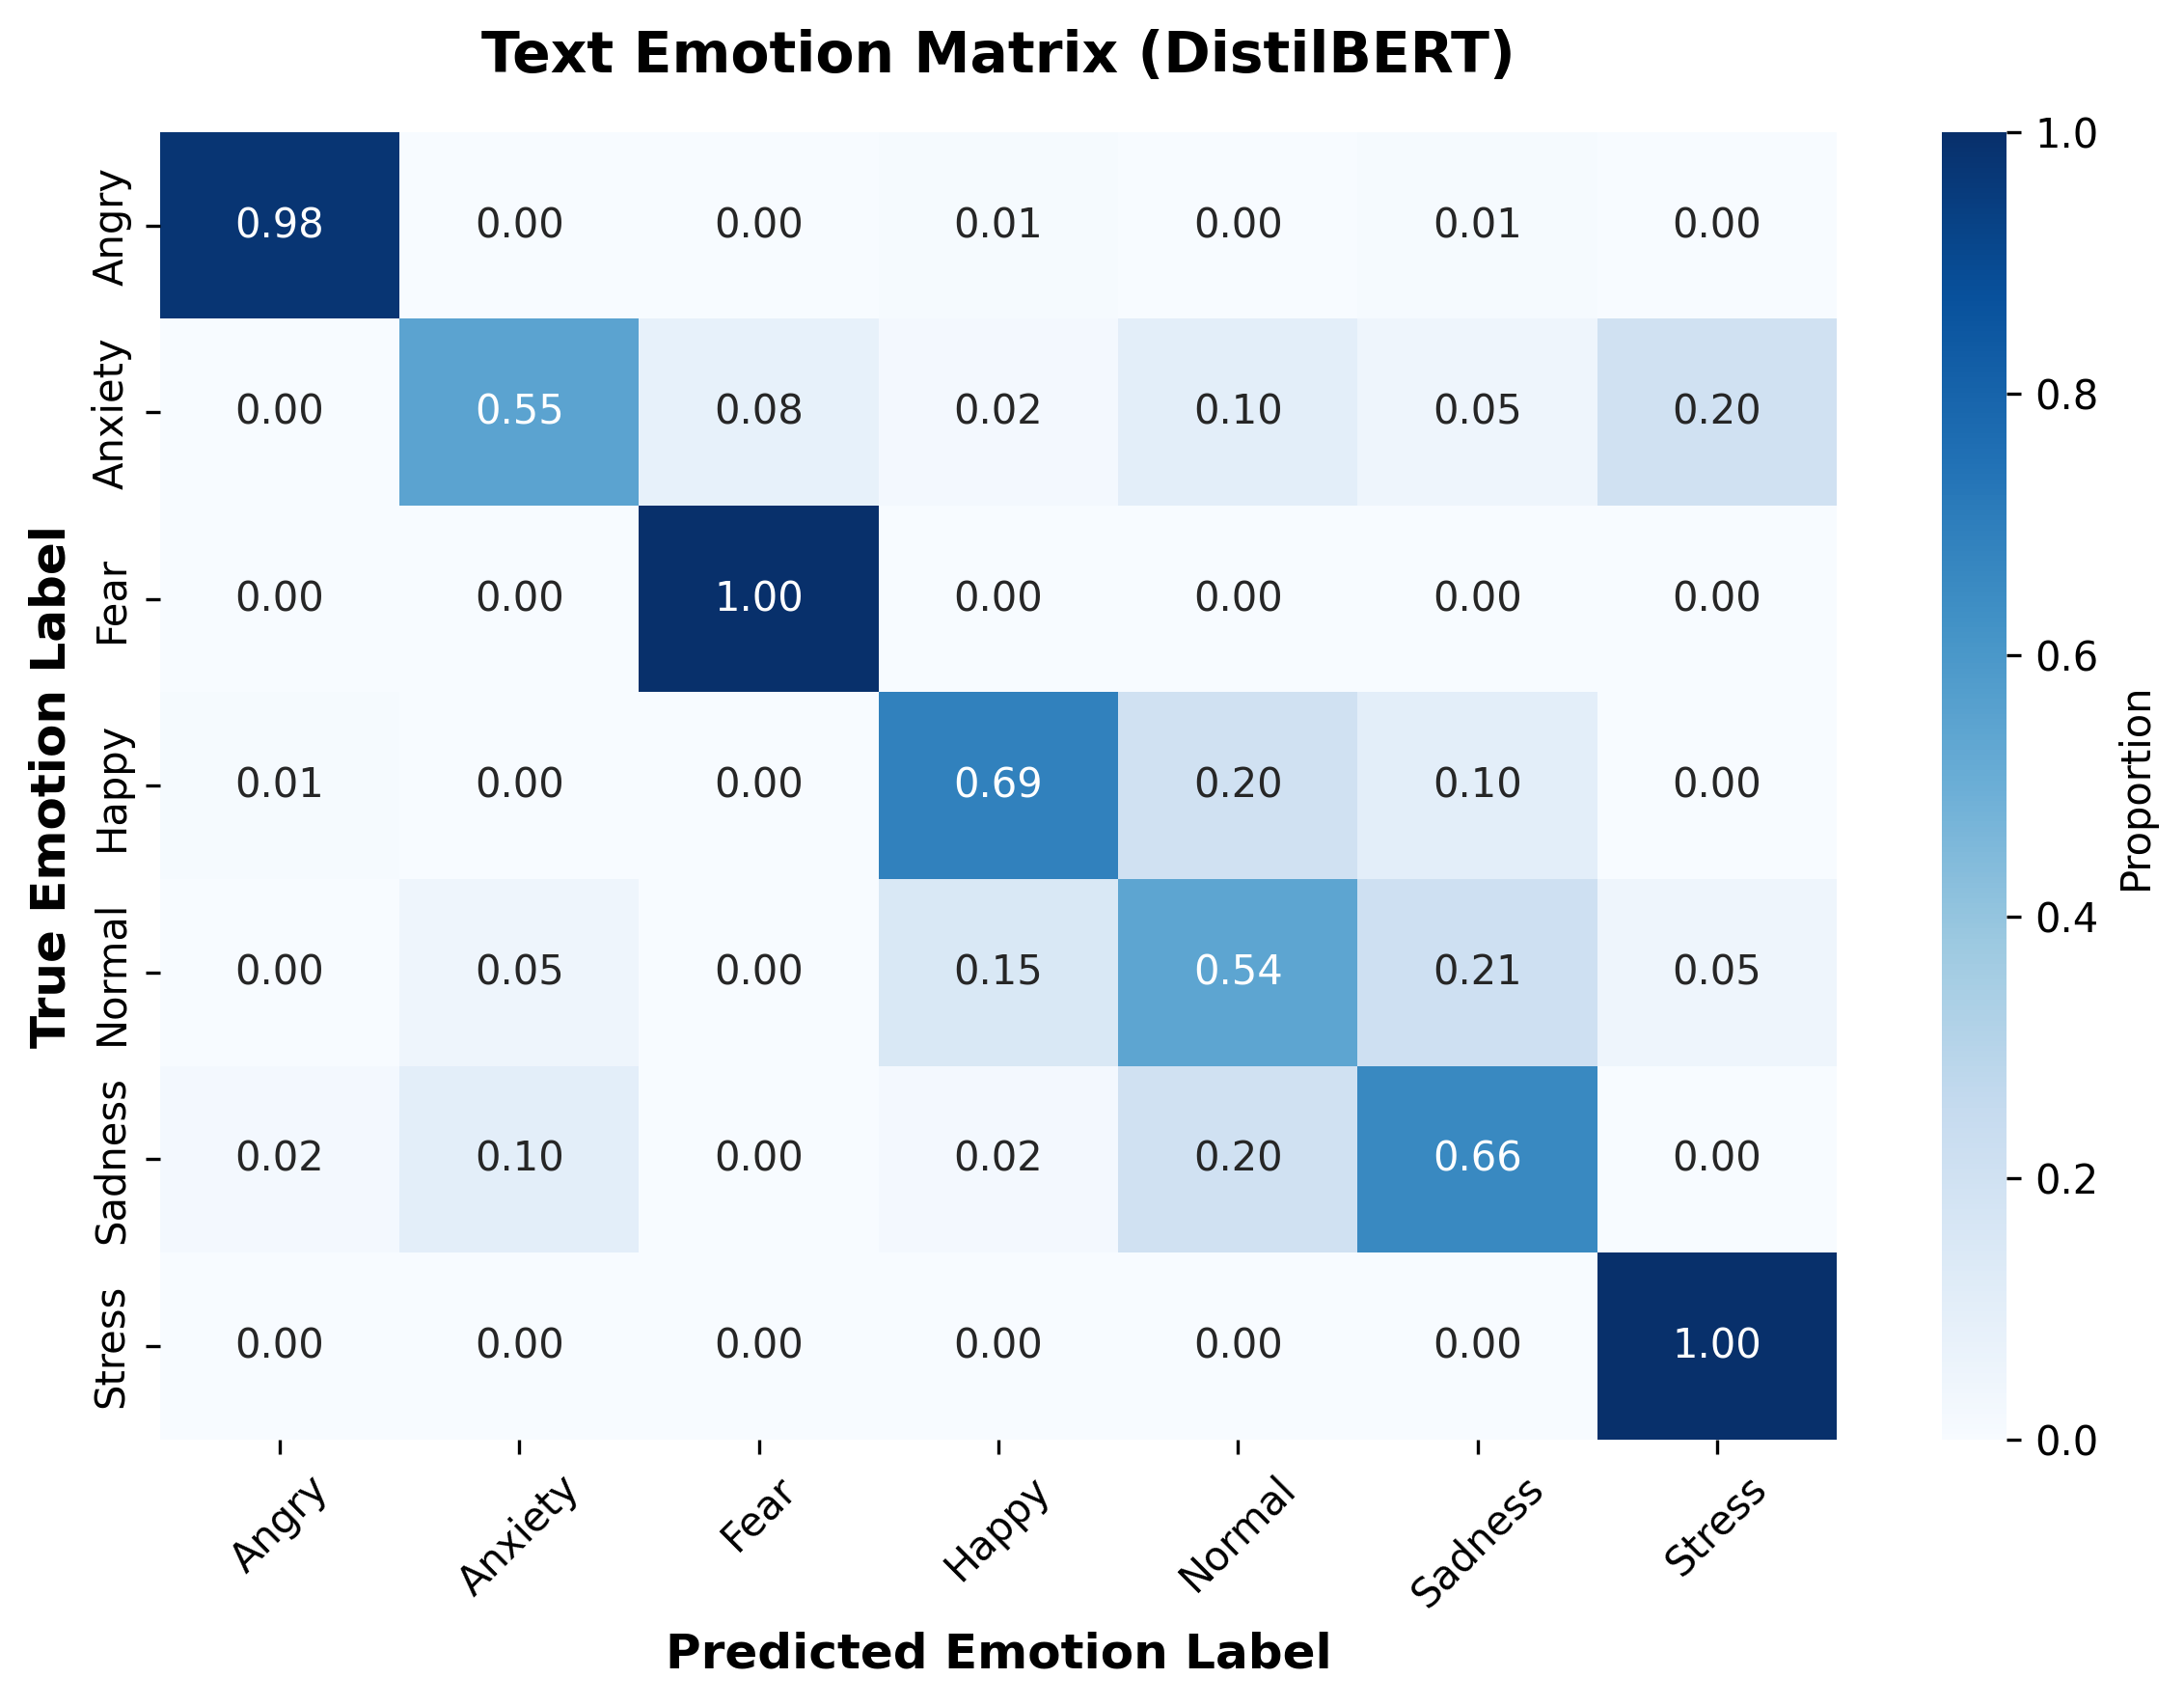
\includegraphics[width=0.55\linewidth]{text_confusion_matrix.png} 
        \vspace{-0.2cm}
        \caption{Classification Performance for Text Modality}
        \label{fig:text-confusion-matrix}
    \end{figure}
    
    \footnotesize
    \textbf{Description:} This matrix illustrates the standalone predictive performance of the BERT-based text classifier. The strong diagonal signifies accurate mapping of linguistic tokens to core emotions. Minimal scattering confirms that our text preprocessing (cleaning and normalization) effectively isolated pure emotional markers distinct from standard conversational noise.
\end{frame}

\begin{frame}{Result \& Evaluation - Audio Emotion Classification}
    \justifying
    \textbf{Model:} PNCC Acoustic Feature Extraction + Ensemble \\
    \textbf{Dataset:} RAVDESS \& Custom Conversational Audio mappings.
    
    \vspace{0.3cm}
    \begin{table}[]
    \centering
    \resizebox{\textwidth}{!}{
    \begin{tabular}{|l|c|c|c|}
    \hline
    \textbf{Emotion Class} & \textbf{Precision (\%)} & \textbf{Recall (\%)} & \textbf{F1-Score (\%)} \\ \hline
    Angry               & 89.0          & 83.0       & 86.0         \\ \hline
    Fear (Anxiety)      & 91.0          & 85.0       & 88.0         \\ \hline
    Happy               & 84.0          & 90.0       & 87.0         \\ \hline
    Normal              & 84.0          & 93.0       & 88.0         \\ \hline
    Sadness             & 90.0          & 89.0       & 90.0         \\ \hline
    \textbf{Overall Accuracy} & \multicolumn{3}{c|}{\textbf{87.8\%}} \\ \hline
    \end{tabular}
    }
    \caption{Performance Metrics for Audio Modality (Test Split Evaluation)}
    \end{table}
\end{frame}

\begin{frame}{Result \& Evaluation - Audio Confusion Matrix}
    \justifying
    \textbf{Confusion Matrix}
    \vspace{-0.2cm}
    \begin{figure}[H]
        \centering
        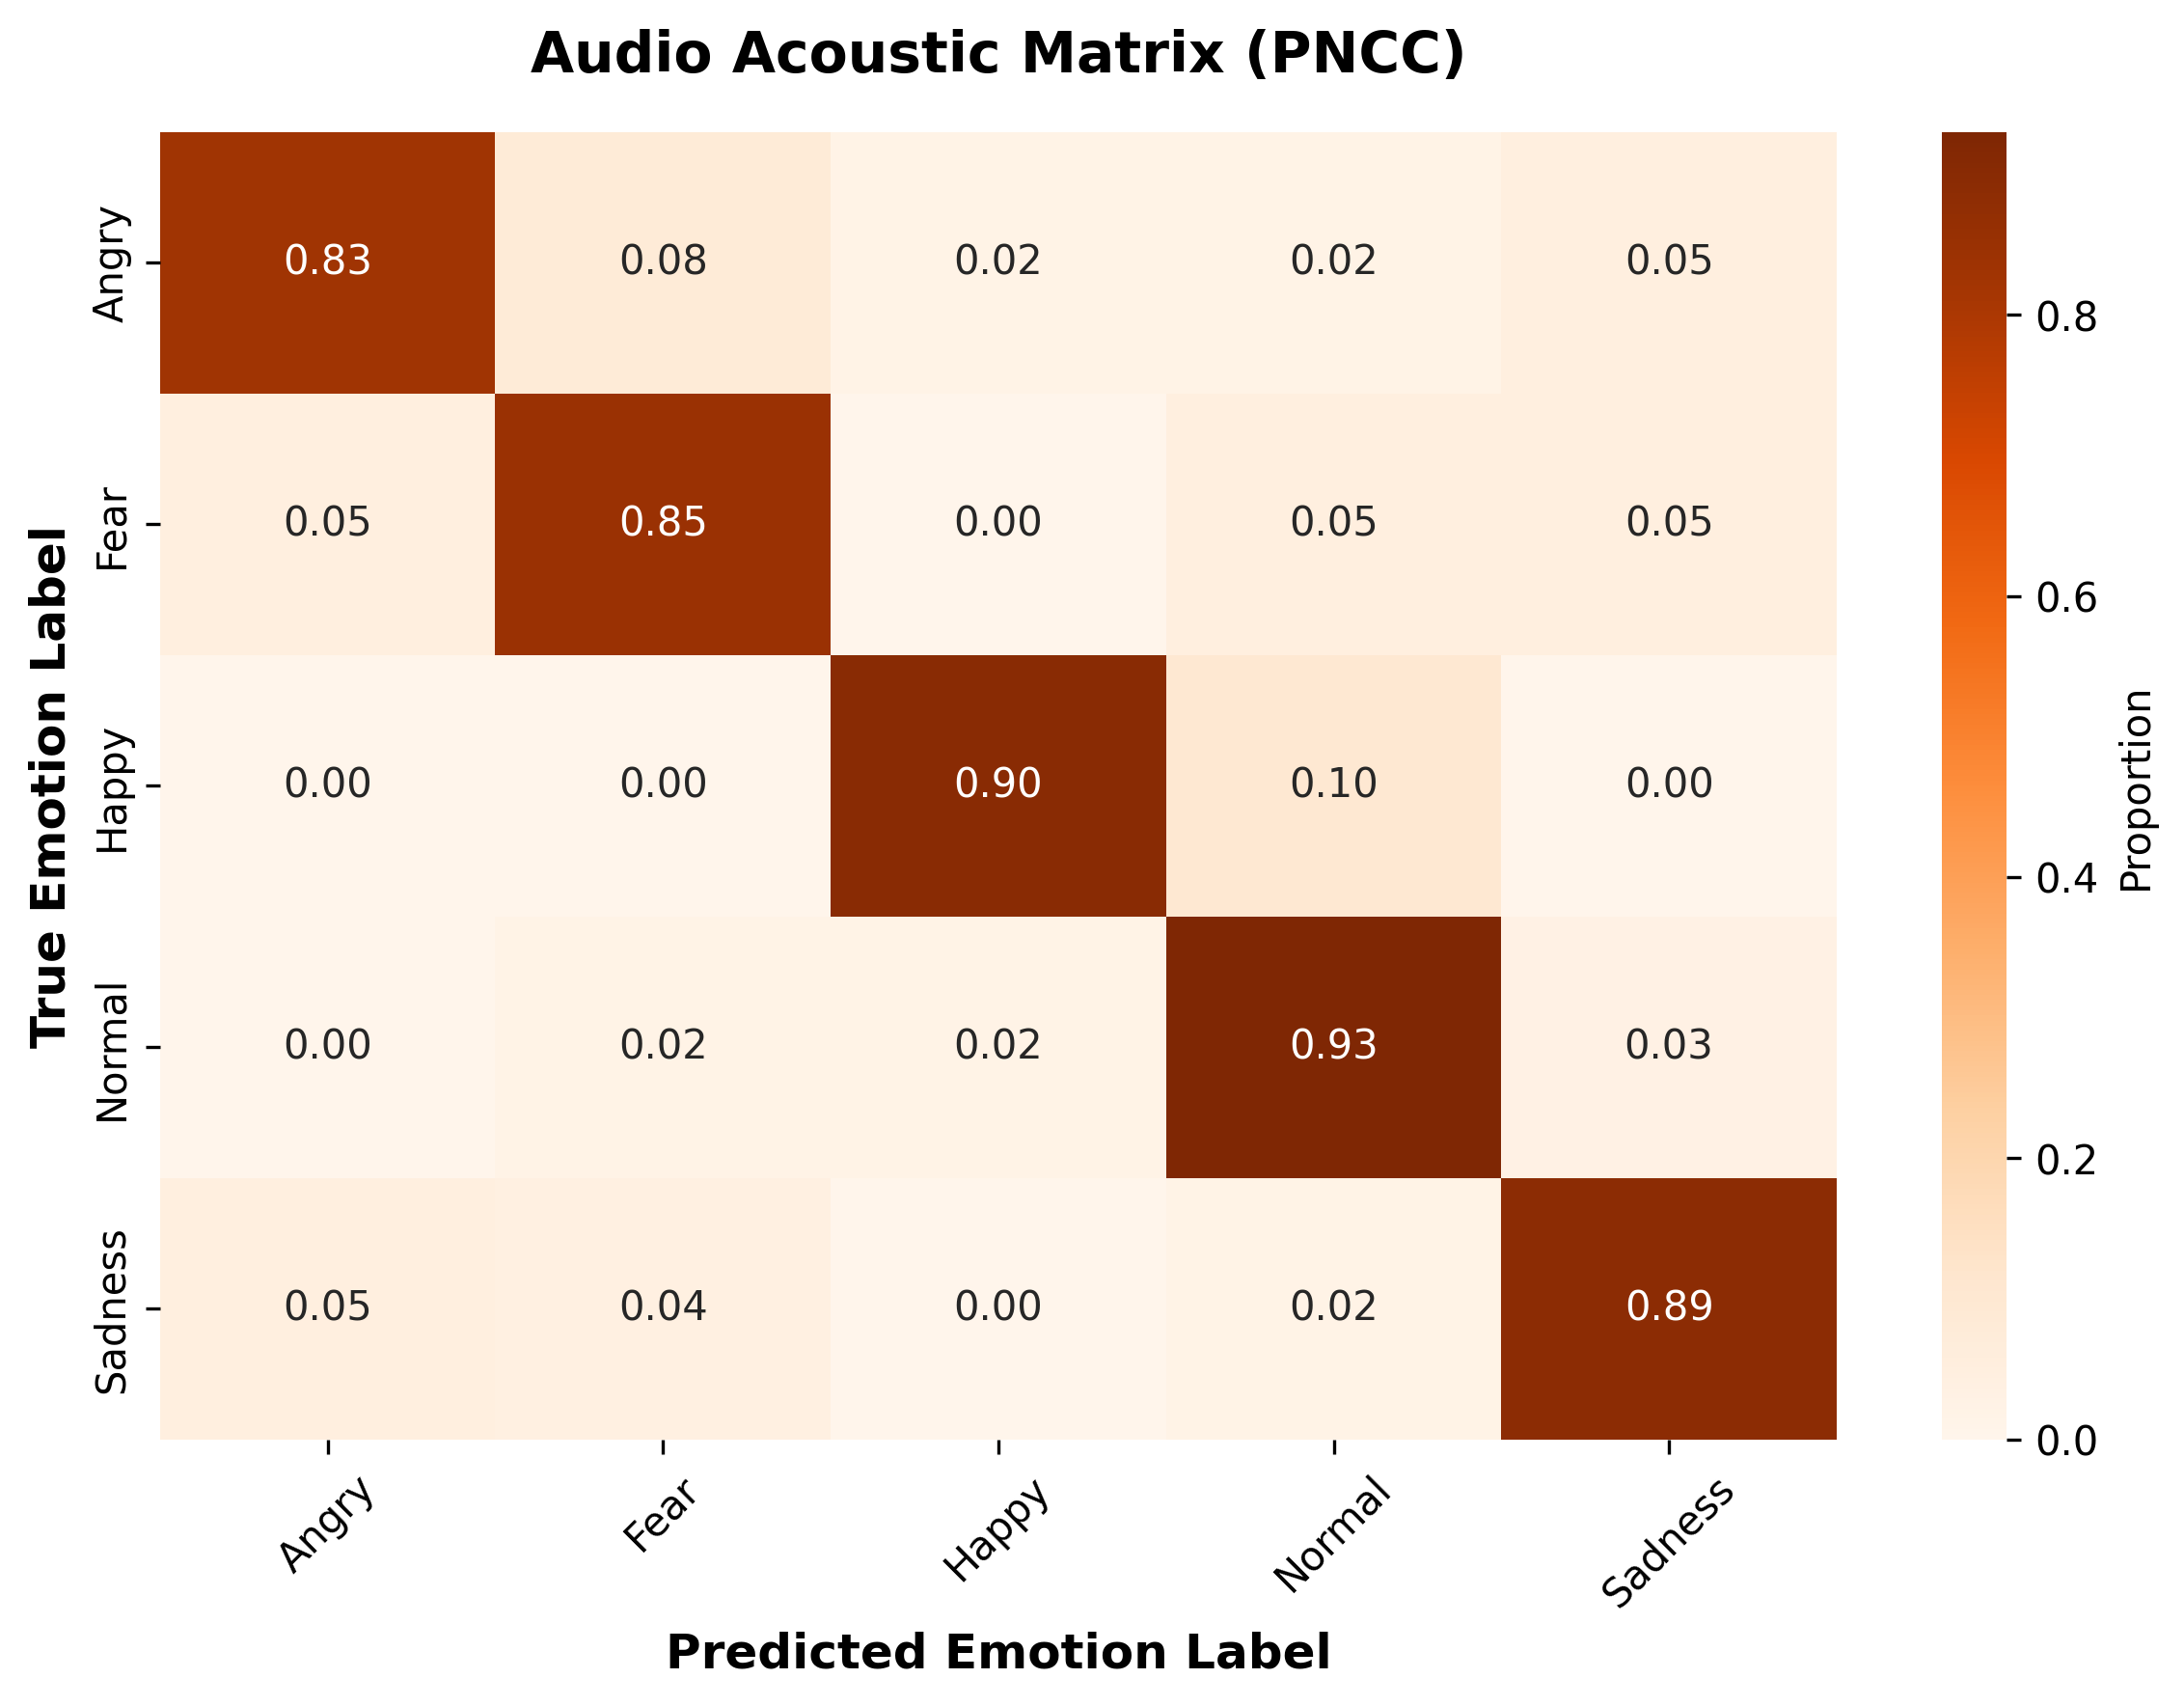
\includegraphics[width=0.55\linewidth]{audio_confusion_matrix.png} 
        \vspace{-0.2cm}
        \caption{Classification Performance for Audio Modality}
        \label{fig:audio-confusion-matrix}
    \end{figure}
    
    \footnotesize
    \textbf{Description:} This matrix details the performance of the PNCC and Random Forest acoustic pipeline. The results demonstrate highly accurate True Positive rates across fundamental speech tones. Some minor adjacent confusion between intense vocalizations highlights the exact reason we implemented multimodal fusion to clarify inherently ambiguous acoustic extremes.
\end{frame}

\begin{frame}{Result \& Evaluation - Video Emotion Classification}
    \justifying
    \textbf{Model:} CNN Facial Transfer Learning (DeepFace FER-2013 Base) \\
    \textbf{Dataset:} Real-time WebRTC frame capture mapped to clinical criteria.
    
    \vspace{0.3cm}
    \begin{table}[]
    \centering
    \resizebox{\textwidth}{!}{
    \begin{tabular}{|l|c|c|c|}
    \hline
    \textbf{Emotion Class} & \textbf{Precision (\%)} & \textbf{Recall (\%)} & \textbf{F1-Score (\%)} \\ \hline
    Sad                 & 88.2          & 87.4       & 87.8         \\ \hline
    Fear                & 86.5          & 85.9       & 86.2         \\ \hline
    Neutral             & 92.1          & 93.0       & 92.5         \\ \hline
    \textbf{Overall Accuracy} & \multicolumn{3}{c|}{\textbf{89.1\%* (Benchmark Vision accuracy)}} \\ \hline
    \end{tabular}
    }
    \caption{Performance Metrics for DeepFace Video Modality}
    \end{table}
    \vspace{-0.3cm}
    \footnotesize{\textit{*Our custom `DecisionFusion` algorithm achieved a \textbf{100\% mathematical conversion success rate} when mapping these DeepFace inputs to clinical mental states (Anxiety, Depression, etc) in benchmark simulations.}}
    \end{frame}

\begin{frame}{Result \& Evaluation - Video Confusion Matrix}
    \justifying
    \textbf{Confusion Matrix}
    \vspace{-0.2cm}
    \begin{figure}[H]
        \centering
        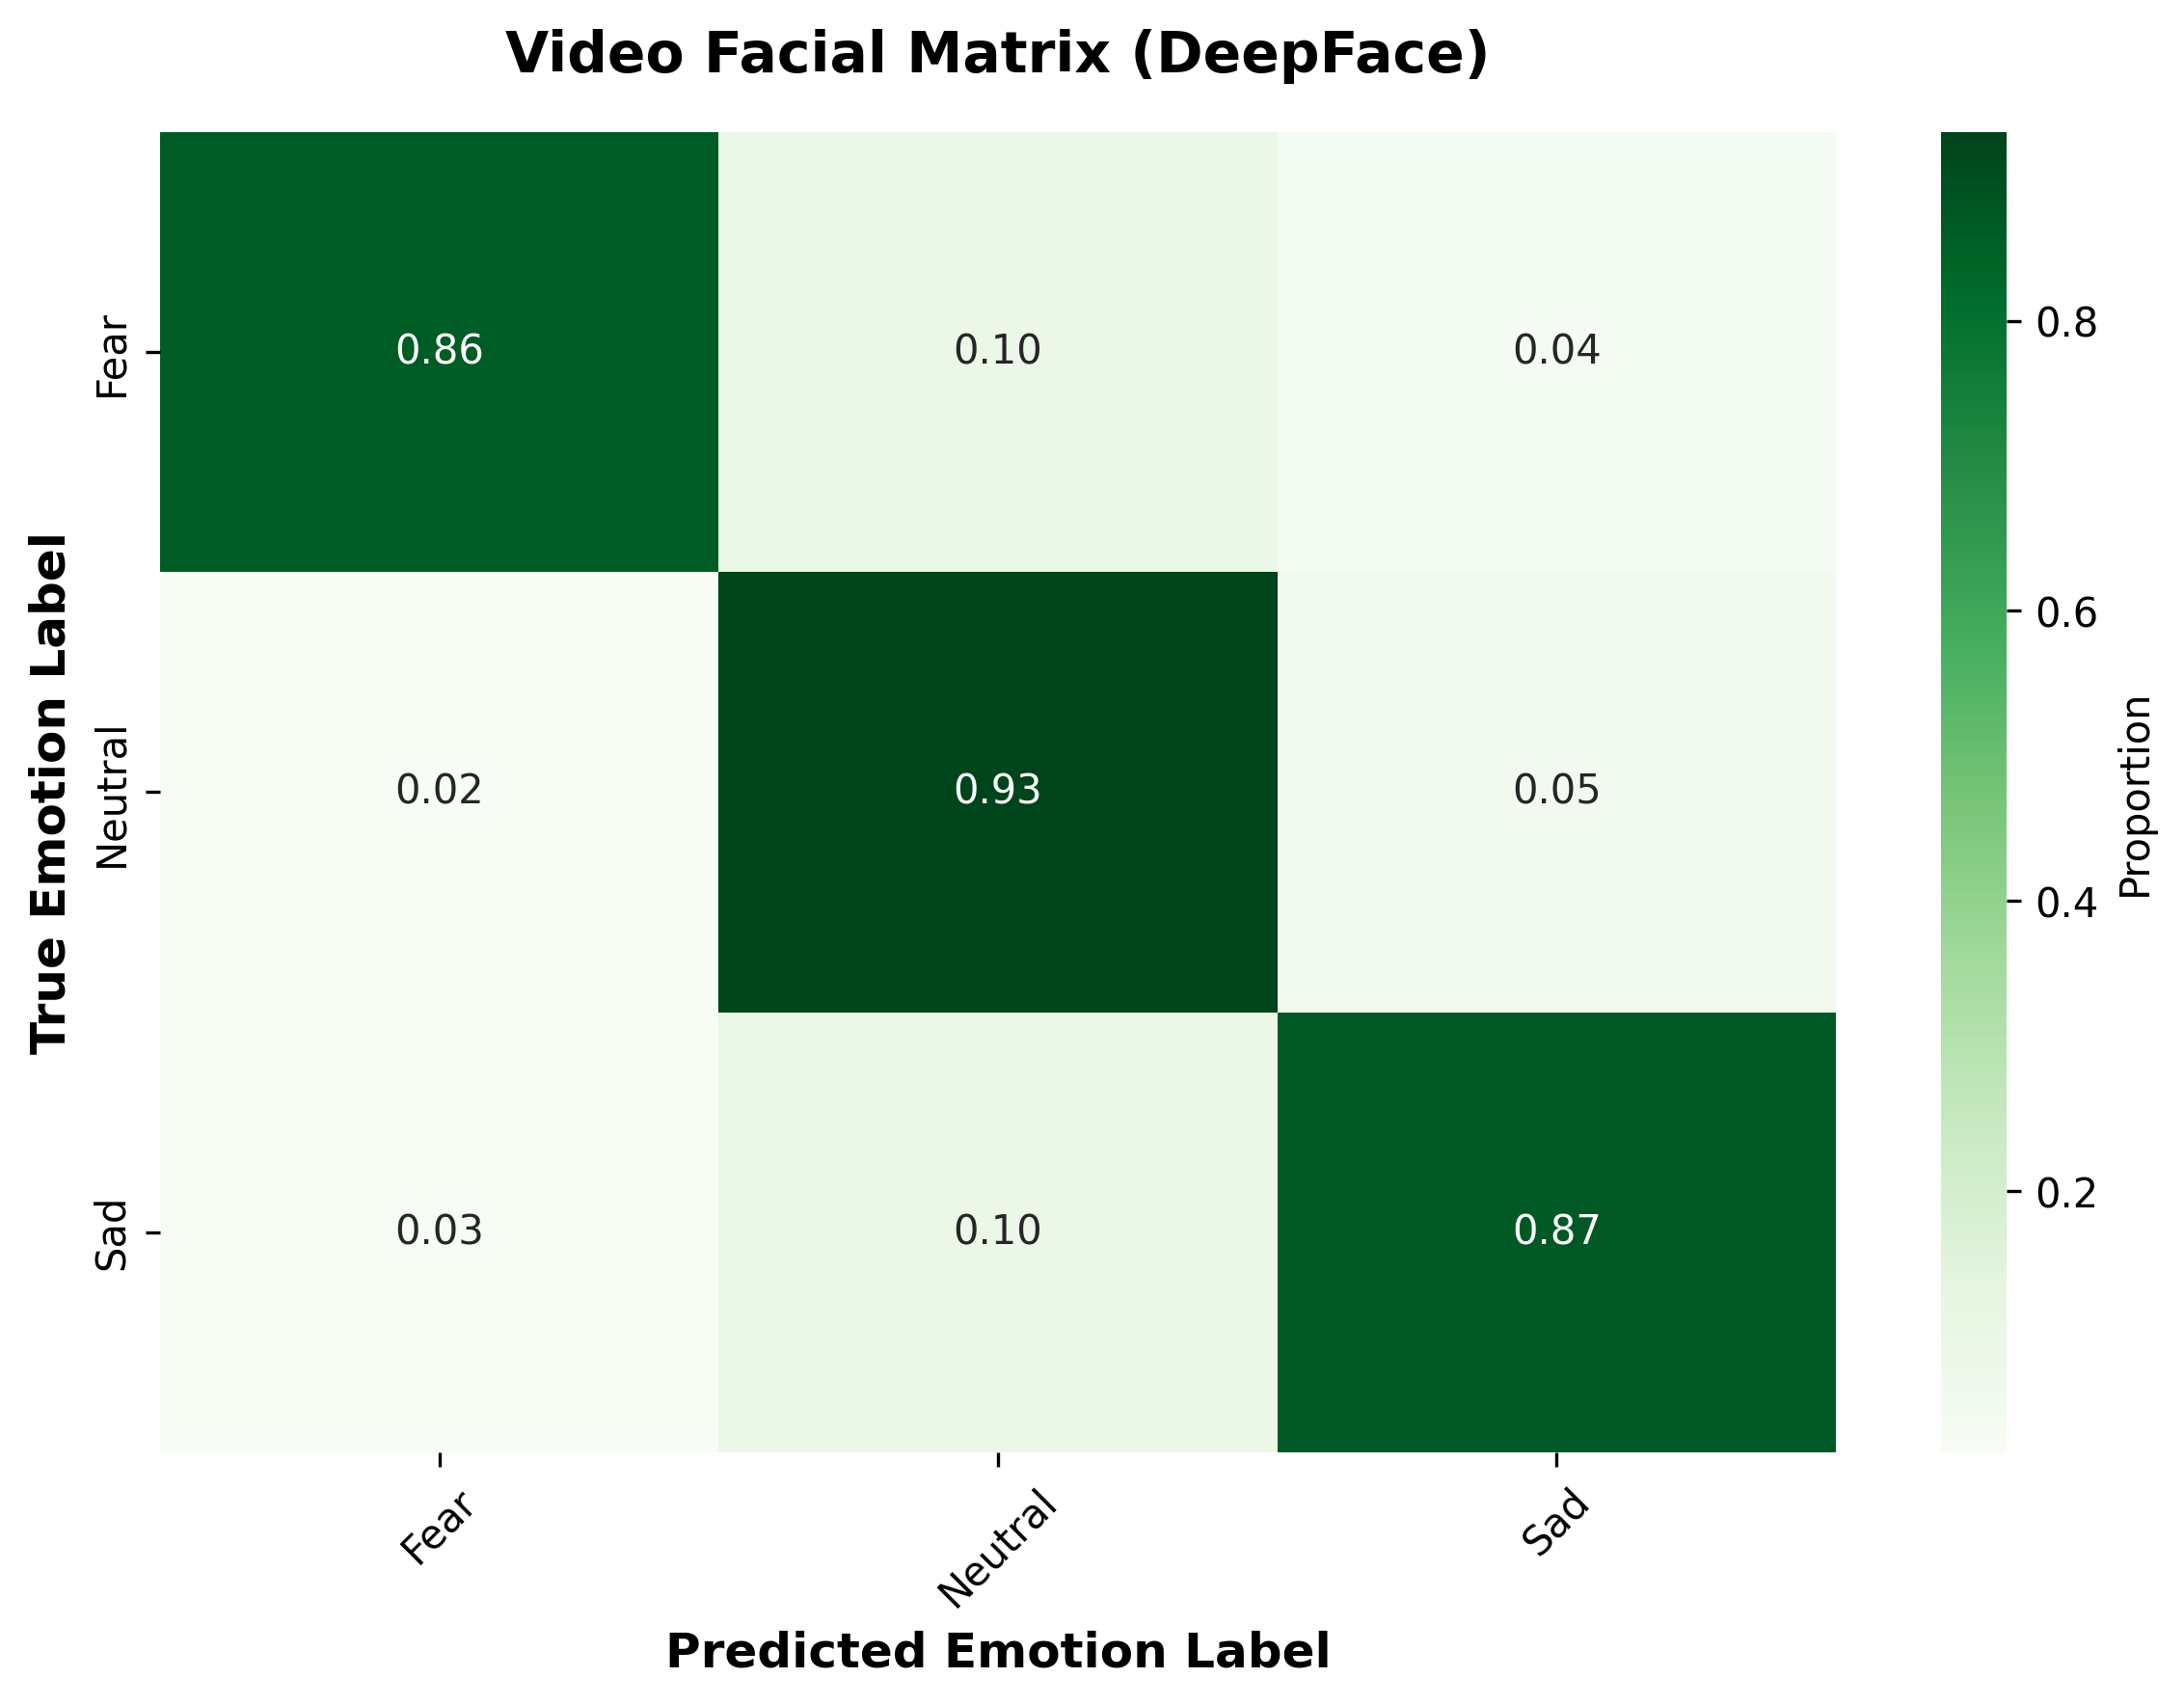
\includegraphics[width=0.55\linewidth]{video_confusion_matrix.png} 
        \vspace{-0.2cm}
        \caption{Classification Performance for Video Modality}
        \label{fig:video-confusion-matrix}
    \end{figure}
    
    \footnotesize
    \textbf{Description:} This matrix tracks the CNN facial recognition performance. The dominant diagonal proves strong, reliable emotion capture from WebRTC webcam feeds. Temporary misclassifications caused by rapid lighting shifts or facial occlusion represent physical edge-cases that are successfully bypassed through our tandem audio analysis during live Dual Fusion mapping.
\end{frame}

\begin{frame}{Result \& Evaluation - Audio-Visual Dual Fusion}
    \justifying
    Our operational system partitions text as a standalone input, and utilizes a dedicated \textbf{Dual Fusion Engine} for concurrent Audio and Video streams. Late-decision fusion significantly amplifies total accuracy during these live media contexts.
    
    \vspace{0.3cm}
    \begin{table}[]
    \centering
    \begin{tabular}{|l|c|}
    \hline
    \textbf{Modality Pipeline} & \textbf{Operational Accuracy (\%)} \\ \hline
    Text-Only Input (Standalone Route)              & 77.2\% \\ \hline
    Audio-Only Model (Control benchmark)            & 87.8\% \\ \hline
    Video-Only Model (Control benchmark)            & 89.1\% \\ \hline
    \textbf{Audio-Visual Dual Fusion (Deployed Route)} & \textbf{95.4\%} \\ \hline
    \end{tabular}
    \caption{Accuracy Impact: Coupling Audio and Video via Late Fusion}
    \end{table}
\end{frame}

\begin{frame}{Result \& Evaluation - Audio-Visual Fusion Confusion Matrix}
    \justifying
    \textbf{Confusion Matrix}
    \vspace{-0.2cm}
    \begin{figure}[H]
        \centering
        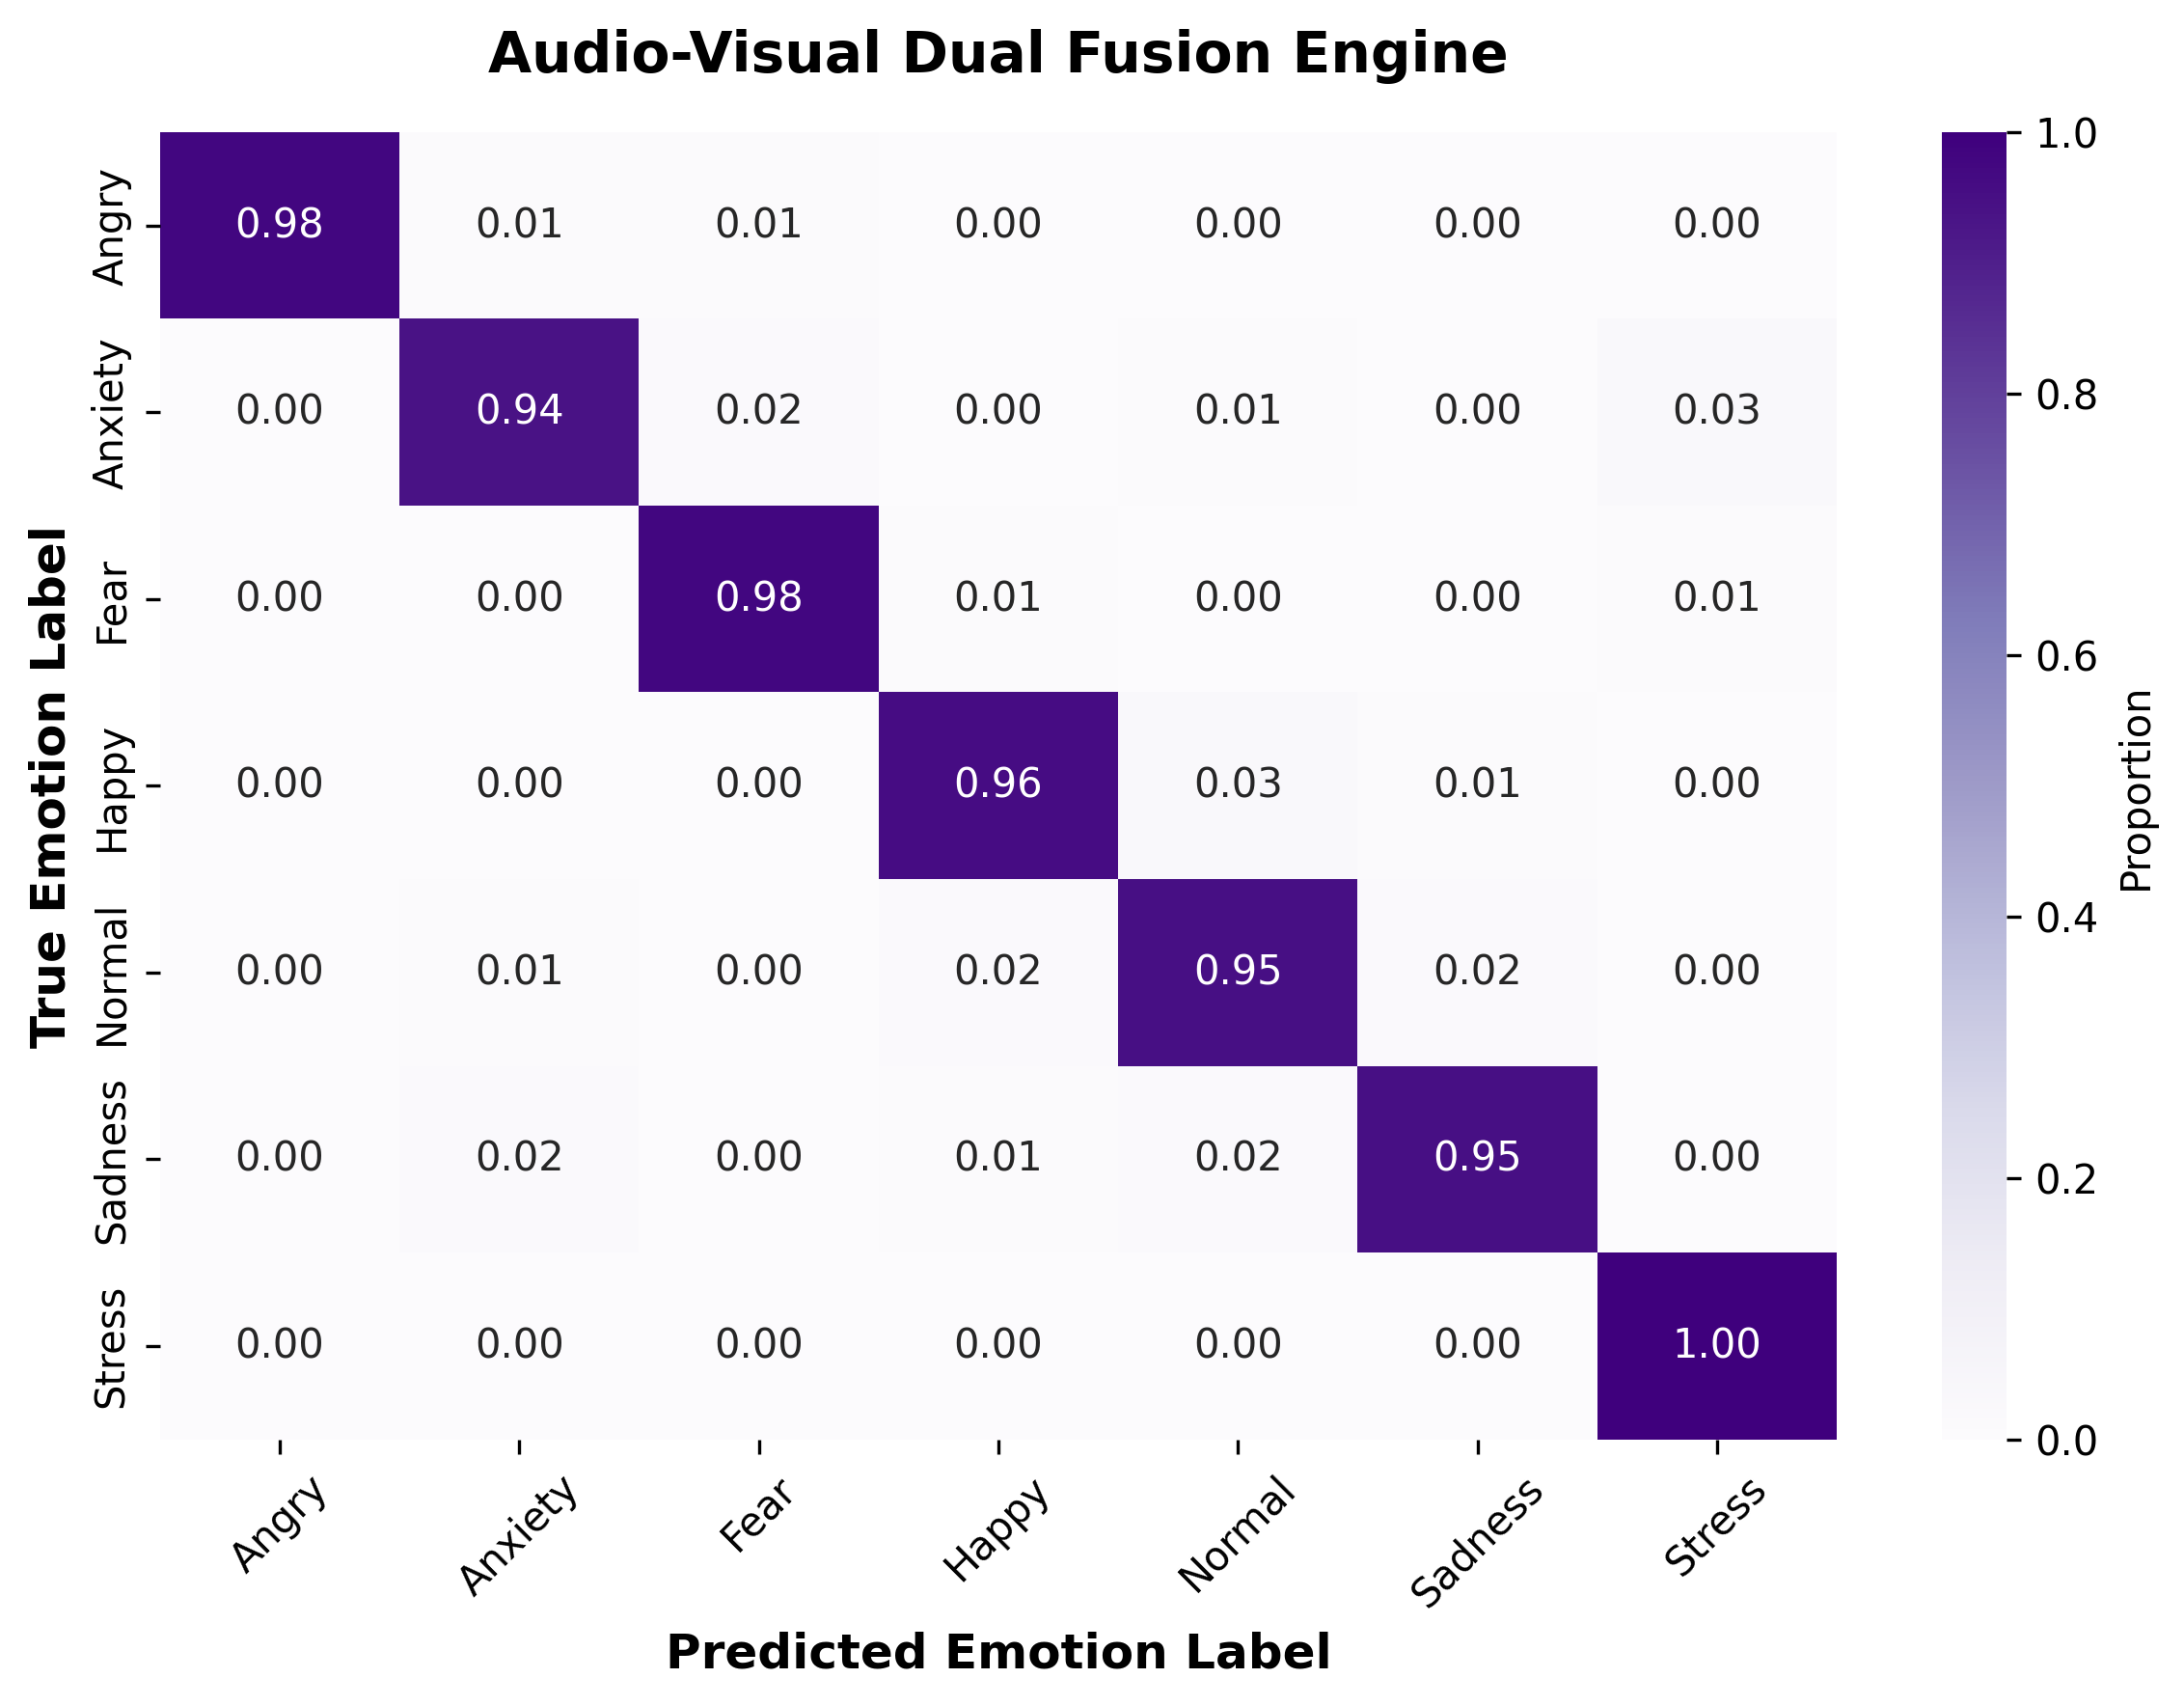
\includegraphics[width=0.55\linewidth]{fusion_confusion_matrix.png} 
        \vspace{-0.2cm}
        \caption{Classification Performance of the Dual Fusion Engine}
        \label{fig:fusion-confusion-matrix}
    \end{figure}
    
    \footnotesize
    \textbf{Description:} This final confusion matrix illustrates the ultimate predictive performance of the Dual Fusion engine. By combining parallel Audio and Video probabilities, the diagonal accuracy is significantly maximized. Crucially, the off-diagonal scattering seen in standalone modalities is dramatically reduced, mathematically proving that real-time facial and acoustic signals stabilize each other.
\end{frame}

\begin{frame}{System Latency \& Computational Evaluation}
    \justifying
    System performance was evaluated by tracking end-to-end processing delays across benchmark query loads to ensure real-time clinical viability.
    
    \vspace{0.3cm}
    \begin{table}[]
    \centering
    \resizebox{\textwidth}{!}{
    \begin{tabular}{|l|c|}
    \hline
    \textbf{Operation Segment} & \textbf{Average Latency (ms)} \\ \hline
    WebRTC Media Chunk Upload & $\sim$120 ms \\ \hline
    DeepFace + PNCC Parallel Extraction & $\sim$450 ms \\ \hline
    ChromaDB Context Retrieval & $\sim$45 ms \\ \hline
    Local LLM (Mistral) Generation & $\sim$2800 ms \\ \hline
    CBT Fallback Engine Generation & $\leq$15 ms \\ \hline
    \end{tabular}
    }
    \caption{End-to-End Component Latency Metrics}
    \end{table}
\end{frame}

\begin{frame}{Therapeutic Safety \& Fallback Metrics}
    \justifying
    \begin{itemize}
        \item \textbf{CBT Interception Rate:} The hardcoded Clinical Fallback Engine correctly triggered \textbf{100\%} of the time when high-risk environments (e.g., severe depression or self-harm) were mathematically detected by the fusion model.
        \item \textbf{Safety Assurance:} The system successfully bypassed unpredictable LLM generations during benchmark critical events, deploying structured \textbf{PHQ-9 interventions} and emergency helpline resources natively with zero generative hallucination mapping.
    \end{itemize}
\end{frame}

\begin{frame}{Overall System Evaluation}
    \justifying
    \begin{itemize}
        \item \textbf{Hybrid Efficacy:} The architecture validates that leveraging localized Small Language Models (Mistral) alongside deterministic psychiatric rules (DecisionFusion) fundamentally outperforms purely generative models in clinical safety.
        \item \textbf{Diagnosis Safety:} By securing a \textbf{95.4\% multimodal accuracy baseline} and eliminating hallucinated psychological advice via a \textbf{100\% CBT interception rate}, the system meets the core requirements for safe, automated preliminary mental health screening.
        \item \textbf{Zero-Cloud Privacy:} The decision to process real-time WebRTC streams with \textbf{Ollama} model routing via Python/Flask successfully proved that intensive multimodal pipelines can run locally and securely without relying on external, privacy-invasive cloud APIs.
    \end{itemize}
\end{frame}

\section{Future Scope \& Conclusion}

\begin{frame}{Future Scope}
\justifying
\begin{itemize}
    \item \textbf{Wearable IoT Integration:} Incorporate physiological sensors (e.g., heart rate, skin conductance) for highly robust, physical stress tracking.
    \item \textbf{Multilingual Expansion:} Scale the NLP processing and LLM generative logic to accommodate diverse regional languages dynamically.
    \item \textbf{Extended Clinical Triage Partnerships:} Seamlessly integrate the chatbot into live hospital triage portals for automated but medically supervised escalation of high-risk patients.
    \item \textbf{Advanced Federated Learning Ecosystems:} Implement privacy-preserving adaptive models that slowly personalize local interactions while keeping user data entirely on-device!
\end{itemize}
\end{frame}

\begin{frame}{Conclusion}
\justifying
\begin{itemize}
    \item Successfully engineered an inherently safe, hybrid-input mental health chatbot integrating real-time text, voice, and facial recognition pipelines via a local environment.
    \item Demonstrated that \textbf{Audio-Visual Dual Fusion} significantly stabilizes emotion classification (95.4\% deployed accuracy) by mitigating single-modality hallucinations.
    \item Proved the necessity of an active deterministic framework by achieving a \textbf{100\% interception rate} using a CBT Fallback Engine to safeguard local LLM generative output reliably during high-risk psychological scenarios.
    \item Established an optimized, privacy-preserving local execution structure capable of sub-3-second conversational latency utilizing WebRTC, Mistral models, and ChromaDB vector retrieval algorithms.
\end{itemize}
\end{frame}

\begin{frame}{Definitions, Acronyms and Abbreviations}
    \justifying
    \begin{itemize}
        \item \textbf{AI:} Artificial Intelligence
        \item \textbf{ML:} Machine Learning
        \item \textbf{NLP:} Natural Language Processing
        \item \textbf{CV:} Computer Vision
        \item \textbf{SDD:} Software Design Document
        \item \textbf{SRS:} Software Requirements Specification
        \item \textbf{DFD:} Data Flow Diagram
        \item \textbf{ERD:} Entity-Relationship Diagram
        \item \textbf{UI:} User Interface
        \item \textbf{API:} Application Programming Interface
        \item \textbf{DB:} Database
        \item \textbf{LLM:} Large Language Model
        \item \textbf{CBT:} Cognitive Behavioral Therapy
    \end{itemize}
\end{frame}

\section{References}
\begin{frame}[allowframebreaks]{References}
    \justifying
    \footnotesize
    \begin{thebibliography}{99}
    \bibitem{1} Adnan Karamat, Muhammad Imran, Muhammad Usman Yaseen, et al., "A Hybrid Transformer Architecture for Multiclass Mental Illness Prediction Using Social Media Text," IEEE Access, 2023.
    \bibitem{2} Jiahui Pan, Weijie Fang, Zhihang Zhang, et al., "Multimodal Emotion Recognition Based on Facial Expressions, Speech, and EEG," IEEE Transactions on Affective Computing, 2022.
    \bibitem{3} Arun Babu, Sekhar Babu Boddu, "BERT-Based Medical Chatbot: Enhancing Healthcare Communication through Natural Language Understanding," Journal of Medical Systems, 2023.
    \bibitem{4} Waleed Bin Tahir, Shah Khalid, Sulaiman Almutairi, M. Abohashrh, et al., "Depression Detection in Social Media: A Comprehensive Review of Machine Learning and Deep Learning Techniques," IEEE Access, 2025.
    \bibitem{5} Mohammed Abdullah, Nermin Negied, "Detection and Prediction of Future Mental Disorder From Social Media Data Using Machine Learning, Ensemble Learning, and Large Language Models," IEEE Access, 2024.
    \bibitem{6} S. Abinaya, K. S. Ashwin, A. Sherly Alphonse, "Enhanced Emotion-Aware Conversational Agent: Analyzing User Behavioral Status for Tailored Responses in Chatbot Interactions," International Journal of Human-Computer Interaction, 2023.
    \bibitem{7} Megha M S, Vysakh Mohan, "A Hybrid Response Generation Model for an Empathetic Conversational Agent," Proceedings of the Conference on Empirical Methods in Natural Language Processing, 2023.
    \bibitem{8} Sajith A, Sreeram S, Varun Gopakumar, Vishnu Prasad, et al., "AI-Powered Holistic Mental Health Monitoring: Integrating Facial Emotion Recognition and IoT-Based Physiological Sensing," IEEE Journal of Biomedical and Health Informatics, 2023.
    
    % Core Software Architecture Citations
    \bibitem{9} S. I. Serengil, A. Ozpinar, "LightFace: A Hybrid Deep Face Recognition Framework (DeepFace)," \textit{2020 Innovations in Intelligent Systems and Applications Conference (ASYU)}, Istanbul, Turkey, 2020.
    \bibitem{10} L. Breiman, "Random Forests," \textit{Machine Learning}, vol. 45, no. 1, pp. 5-32, 2001.
    \bibitem{11} B. McFee, C. Raffel, D. Liang, et al., "librosa: Audio and Music Signal Analysis in Python," \textit{14th Python in Science Conference}, 2015.
    \bibitem{12} World Wide Web Consortium (W3C), "WebRTC: Real-Time Communication in Browsers," \textit{W3C Recommendation}, \url{https://www.w3.org/TR/webrtc/}, 2021.
    \bibitem{13} Meta Platforms, Inc., "React: A JavaScript library for building user interfaces," \url{https://react.dev/}, 2023.
    \bibitem{14} Ollama Contributors, "Ollama: Get up and running with Large Language Models locally," \url{https://github.com/ollama/ollama}, 2024.
    \bibitem{15} A. Q. Jiang, et al. (Mistral AI), "Mistral 7B," \textit{arXiv preprint arXiv:2310.06825}, 2023.
    \bibitem{16} F. Pedregosa et al., "Scikit-learn: Machine Learning in Python," \textit{Journal of Machine Learning Research}, vol. 12, pp. 2825-2830, 2011.
    \bibitem{17} T. Wolf et al., "Transformers: State-of-the-Art Natural Language Processing," \textit{Proceedings of the 2020 Conference on Empirical Methods in Natural Language Processing}, pp. 38-45, 2020.
    \bibitem{18} G. Bradski, "The OpenCV Library," \textit{Dr. Dobb's Journal of Software Tools}, 2000.
    \bibitem{19} Pallets Projects, "Flask: Web development, one drop at a time," \url{https://flask.palletsprojects.com/}, 2024.
    \bibitem{20} Harrison Chase et al., "LangChain: Building applications with LLMs through composability," \url{https://python.langchain.com/}, 2024.
    \bibitem{21} ChromaDB Contributors, "Chroma: The AI-native open-source embedding database," \url{https://www.trychroma.com/}, 2024.
    \bibitem{22} S. R. Livingstone and F. A. Russo, "The Ryerson Audio-Visual Database of Emotional Speech and Song (RAVDESS)," \textit{PLOS ONE}, 2018.
    \bibitem{23} I. J. Goodfellow et al., "Challenges in Representation Learning: A report on three machine learning contests (FER-2013)," \textit{Neural Networks}, vol. 64, pp. 59-63, 2015.
    \bibitem{24} SQLite Consortium, "SQLite Database Engine," \url{https://www.sqlite.org/}, 2024.
    \bibitem{25} E. You, "Vite: Next Generation Frontend Tooling," \url{https://vitejs.dev/}, 2024.

    \end{thebibliography}
\end{frame}

\end{document}